\documentclass[a4paper,11pt]{report}
\usepackage{amssymb}
%%%%%%%%%%%%%%%%%%%%%%%%%%%%%%%%%%%%%%%%%%%%%%%%%%%%%%%%%%%%%%%%%%%%%%%%%%%%%%%%%%%%%%%%%%%%%%%%%%%%%%
% !TEX encoding = UTF-8 Unicode
\usepackage{UFMG_style}
%\usepackage{oxthesis}
\usepackage{etexcmds,epsfig}
\usepackage{amssymb, amsmath, multicol, rotating, xcolor} 
\usepackage{graphicx, balance}
\usepackage{subfigure}% Support for small, `sub' figures and tables
\usepackage{ccaption}
\usepackage{amsfonts}  %% 100
\usepackage{graphics}  %% 100
\DeclareGraphicsExtensions{.pdf,.svg,.eps,.png,.jpg,.jpeg}
\usepackage[portuges]{varioref}
\usepackage[utf8]{inputenc}
\usepackage{url} 
\usepackage[T1]{fontenc}
\usepackage{dirtytalk} % quotations
\usepackage{makeidx}
\usepackage[portuges,brazilian]{babel}
\usepackage{hyphenat}
\usepackage{tabularx,balance,indentfirst}
\setcounter{MaxMatrixCols}{10}
\usepackage{floatrow}
\usepackage{chngcntr}
\usepackage{microtype}
%\usepackage[xindy,toc,acronym]{glossaries}
%%%%%%%%
\makeatletter
\let\X@old@caption\caption
\def\X@caption@minusone{\expandafter\advance\csname c@\@captype\endcsname-1 }
\def\X@caption@br[#1]#2{\X@old@caption[#1]{#2}\X@caption@minusone}
\def\X@caption@nobr#1{\X@old@caption{#1}\X@caption@minusone}
\def\caption{\@ifnextchar[\X@caption@br\X@caption@nobr}
\makeatother
%%%%%%%%
% substitui Verbatim
\usepackage{listings}
\lstset{numbers=left,commentstyle=\color{green},keywordstyle=\color{blue}}
\usepackage{inconsolata}
\lstset{
    language=matlab, %% Troque para PHP, C, Java, etc... bash é o padrão
    basicstyle=\ttfamily\small,
    numberstyle=\footnotesize,
    numbers=left,
    %backgroundcolor=\color{gray!1}, %estava 10
    frame=single,
    tabsize=2,
    rulecolor=\color{black!30},
    title=\lstname,
    escapeinside={\%*}{*)},
    breaklines=true,
    breakatwhitespace=true,
    framextopmargin=2pt,
    framexbottommargin=2pt,
    extendedchars=false,
    showstringspaces=false,
    inputpath=./programas/,
    %inputencoding=utf8
}
%------------------------------------------------------%
\newtheorem{teorema}{Teorema}
\newtheorem{algoritmo}{Algoritmo}
\newtheorem{axioma}{Axioma}
\newtheorem{caso}{Caso}
\newtheorem{conclusão}{Conclusão}
\newtheorem{condição}{Condição}
\newtheorem{conjectura}{Conjectura}
\newtheorem{corol\'{a}rio}{Corol\'{a}rio}
\newtheorem{crit \'{e}rio}{Crit \'{e}rio}
\newtheorem{definicao}{Definicao}
\newtheorem{definição}{Definição}
\newtheorem{exemplo}{Exemplo}
\newtheorem{exerc\'{\i}cio}{Exerc\'{\i}cio}
\newtheorem{lema}{Lema}
\newtheorem{nota\c{c}\~{a}o}{Nota\c{c}\~{a}o}
\newtheorem{observa\c{c}\~{a}o}{Observa\c{c}\~{a}o}
\newtheorem{problema}{Problema}
\newtheorem{proposi\c{c}\~{a}o}{Proposi\c{c}\~{a}o}
\newtheorem{solu\c{c}\~{a}o}{Solu\c{c}\~{a}o}
\newtheorem{resumo}{Resumo}
\newenvironment{prova}[1][Prova]{\textbf{#1.} }{\ \rule{0.5em}{0.5em}}
\renewcommand{\baselinestretch}{1.2}  
\setcounter{tocdepth}{2} 
\newcommand{\bref}[1]{\mbox{(\ref{#1})}}
%-------------------------------------------------------%
\counterwithin{figure}{chapter}
\counterwithin{exemplo}{chapter}
\counterwithin{definição}{chapter}
\counterwithin{algoritmo}{chapter}


% If dedication remove the next line comment...
%\dedication{Para ...}

\college{Minha Unidade}  
\advisor{Orientador: Prof.  Fulano de Tal, UFMG \\
Supervisor: Eng. John Doe, Empresa}
\fulfilment{Relatório de Estágio Técnico do Projeto PRAE/COLTEC/UFMG} 

%\fulfilment{Monografia submetida à banca examinadora designada pelo Colegiado Didático do Curso de Graduação em Engenharia de Controle e Automação da Universidade Federal de Minas Gerais, como parte dos requisitos para aprovação na disciplina Projeto Final de Curso II} 

\submitterm{Novembro,}
\submityear{2017}

%\draft


%%%%%%%%%%%%%%%%%%%%%%%%%%%%%
% INICIO
%%%%%%%%%%%%%%%%%%%%%%%%%%%%%

\begin{document}
% Título...
\title{Título com assunto e proposta}
\author{Autor Nome Sobrenome}
\maketitle

%\input{capa}

\pagenumbering{roman} % Use Roman numbers for the frontmatter pages.

\begin{abstract}
%\input{abstract}
% !TEX encoding = UTF-8 Unicode
%\section{Abstract}

O resumo deve explicitar o assunto, a proposta e o escopo do trabalho. Ao ler o resumo o leitor deve entender de que se trata efetivamente o trabalho ou projeto, o que se aborda e como se produz evidências (simulação, experimento, dedução teórica). Normalmente a última sentença do resumo trata das evidências e discussões apresentadas ou almejadas. 


\end{abstract}

\tableofcontents
\listoffigures

\begin{acknowledgements}
%%%%%%%%%%%%%%%%%%%%%%%%%%%%%%%%%%%%%
%% Agradecimentos
%%%%%%%%%%%%%%%%%%%%%%%%%%%%%%%%%%%%%
% !TEX encoding = UTF-8 Unicode
\arb[PARA DELETAR:]{Para editar o texto a seguir faça-o no arquivo em separado: \texttt{agradecimentos.tex}  }


Lembre-se de agradecer o seu orientador, supervisor, agências de fomento ou financiamento (FUMP, CNPq, FAPEMIG, Empresa XYZ, etc.), e colegas que eventualmente te ajudaram a realizar este trabalho. 

Este espaço não é lugar adequado para você agradecer  a sua existência e todo mundo que você conhece e que  te ajudou desde que você existe (use o Agradecimentos para mencionar quem  contribuiu especificamente para realizar este trabalho!).

Agradecer a quem te sustentou financeiramente (familiares, amigos, tutores) ou emocionalmente (evite citar quem você pode querer apagar depois!) é usual, mas por favor, sem detalhar sua história de vida!	 % File with my agradecimentos.tex   (same folder of master)
\end{acknowledgements}

\pagenumbering{arabic} % Use arabic numbers for the mainmatter.

% Subpastas para cada capítulo
% !TEX encoding = UTF-8 Unicode
\graphicspath{{figuras/}}

\chapter{Introdução \label{cap1}}

O Relatório Técnico Final é um documento em que o leitor encontra todas as informações técnicas sobre o trabalho desenvolvido. 
O relatório deve conter os seguintes tópicos:
\begin{itemize}\item {\bf Capa ou página de título: } deve conter o nome da instituição, o título (e subtítulo) do projeto, os autores e supervisores, local e data. O título é considerado o resumo mais sintético do projeto e, portanto, é imprescindível que inclua o assunto ou o tópico e a proposta do mesmo. Verifique ainda se o título é: suficientemente preciso, fácil para ler e entender, e  estruturado para o tema e a audiência. 
\item {\bf Contra-capa: } mesma informação da capa mais as assinaturas dos autores.
\item {\bf Sumário: } Enumeração das principais divisões (capítulo, seções, artigos, etc.) do documento, na mesma ordem em que a matéria nele se sucede; visa a facilitar visão do conjunto da obra e a localização de suas partes, e, para tanto, deve aparecer no início da publicação e indicar, para cada parte, a paginação (Dicionário Aurélio, 1999).
\item {\bf Abstract:} é um resumo sucinto do trabalho que serve como um guia para a leitura do relatório. A leitura do abstract deve indicar se vale ou não a pena ler o relatório. 
O abstract pode ser de dois tipos:

\begin{itemize}
  \item Abstract descritivo que responde a questão: qual é o escopo do relatório?
    \item Abstract informativo que responde a questão: quais são os pontos mais importantes apresentados no relatório.
\end{itemize}

\item {\bf Introdução:} uma introdução bem escrita deve abordar os seguintes itens:
  \begin{itemize}
  	\item o assunto  	\item a proposta ou proposição
	\item Objetivos: 
	Enumere uma lista com bullets. Recomenda-se iniciar os itens com verbos no infinitivo. É imperativo manter o paralelismo de linguagem, i.e. se o primeiro item inicia-se com um verbo no infinitivo, todos os demais itens devem também iniciar com verbos no infinitivo!
  	\item o "background" ou fundamentos do projeto  	\item o escopo  	\item a organização do relatório 	 \item os termos chaves
  \end{itemize}
	  \item {\bf Descrição da metodologia:} descreva os métodos usados para executar o projeto.  \item {\bf Apresentação dos resultados}  \item {\bf Conclusões:} conclua baseado nos resultados apresentados, comentando todos os objetivos propostos.  \item {\bf Sugestões e recomendações}  \item {\bf Apêndices:} nomenclatura utilizada (vide exemplo) e material de suporte ou complementação do corpo do relatório, e.g. diagramas de circuitos, códigos de programas desenvolvidos, etc.  \item {\bf Referências bibliográficas}.
\end{itemize}

Um livro clássico mas difícil de ler e entender é \cite{Astrom:1970}, mas também clássico e muito bom é \cite{Astrom:1997}.

Note que figuras são referenciadas com o rótulo {\it figura} seguindo de uma referência numérica sem parênteses, e.g. Mostra-se na figura \ref{fig_cap1_MBPC_blk_diag} um diagrama em blocos de uma arquitetura de controle de processos genérica.

A referência a uma equação é feita usando numeração entre parênteses, e.g. a equação \bref{eq_piuBella} é uma das mais belas equações matemáticas.

\begin{equation}
 \frac{dy}{dt} = A y.   
 \label{eq_piuBella}
\end{equation}


\begin{figure}[!htbp]
\centering
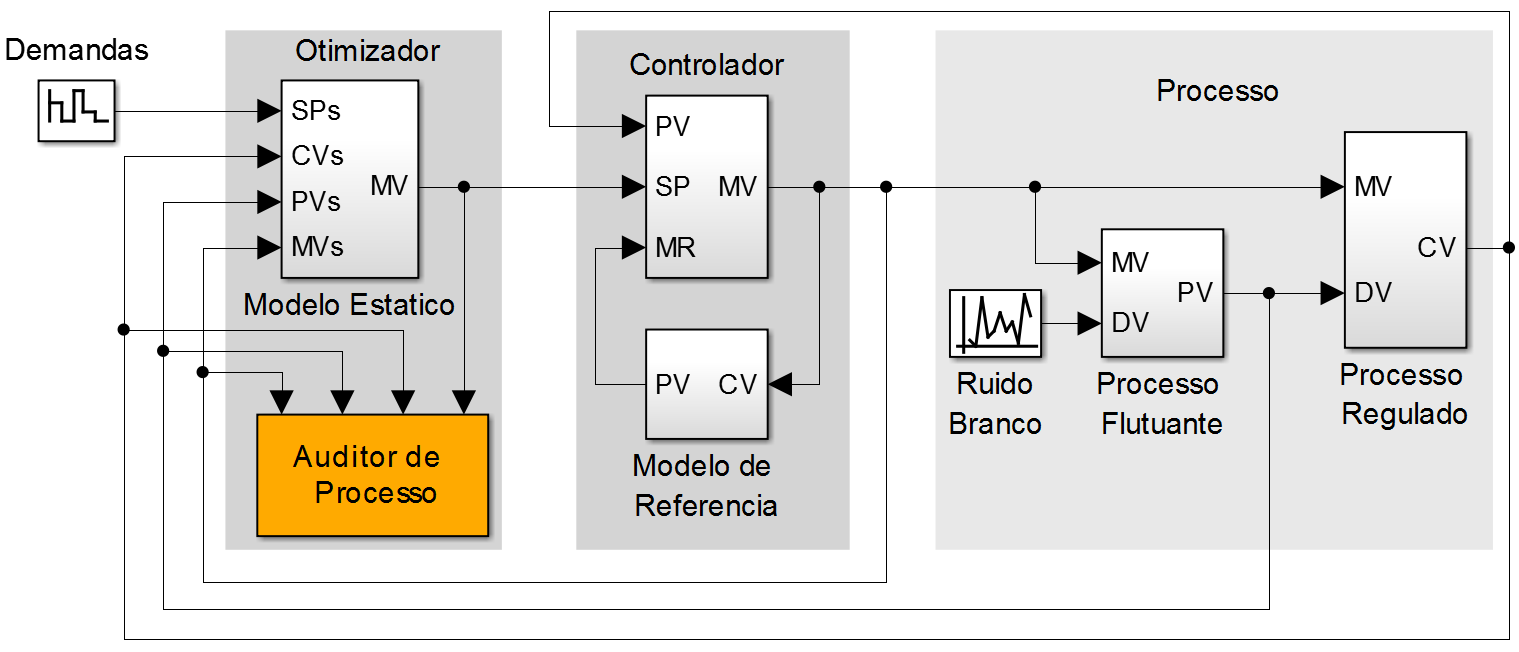
\includegraphics[width=15cm]{cap1_MBPC_blk_diag} 
\caption{Arquitetura simplificada de um sistema de controle baseado em modelo com a função de Auditor de Processo.}
\label{fig_cap1_MBPC_blk_diag}
\end{figure}


\section{Contribuições}

As principais contribuições apresentadas neste trabalho são destacadas abaixo para cada capítulo.

\begin{itemize}

  \item \textbf{Capítulo \ref{cap1}}. Neste capítulo contribuiu-se a partir de uma revisão da literatura...
  
  \item \textbf{Capítulo \ref{cap2}}. Descreve-se...
  
  \item \textbf{Capítulo \ref{cap3}}. Apresenta-se...
  
  \item \textbf{Capítulo \ref{cap4}}. No capítulo 4 é apresentada ...
  
  \item \textbf{Capítulo \ref{cap5}}. No capítulo 5 é apresentada ...
  
\end{itemize}


Conclusões e sugestões de trabalho futuro são apresentadas no Capítulo \ref{cap6}.

% !TEX encoding = UTF-8 Unicode
\graphicspath{{figuras/}}

\chapter{Título do capitulo 2}
\label{cap2}

Texto resumo introdutório do capítulo...

\section{Introdução}


\section{Comentários finais}

% !TEX encoding = UTF-8 Unicode
\graphicspath{{figuras/}}


% !TEX encoding = UTF-8 Unicode

\chapter{Recomendações para elaboração de proposta de projeto}
\label{cap3}


O trabalho com o desenvolvimento de projetos propicia uma oportunidade de aprender a fazer planejamentos com o propósito de transformar uma ideia em realidade, de resolver um problema concreto (\cite{Signorelli2001}). Possibilita, ainda, ensinar de uma forma pragmática a elaborar cronogramas com objetivos parciais nos quais o trabalho rumo aos objetivos finais é avaliado permanentemente de modo a corrigir erros de processo ou mesmo de planejamento conforme ilustrado na Figura~\ref{fig:fluxogramaDeProjeto}. Espera-se que o estudante aprenda a planejar e implementar projetos, analisando dados, ponderando situações e tomando decisões. O fundamental é que o estudante tenha a oportunidade de imaginar uma ação, traçar um plano para torná-la real num tempo predeterminado, realizar esse plano, controlar o processo, responder aos acontecimentos imprevistos e chegar ao resultado esperado. O mais  importante ao final do trabalho é se houve aprendizado e não se um determinado produto ficou belíssimo ou encapsulado profissionalmente. O texto técnico que relata o desenvolvimento do projeto é normalmente corrigido pelo orientador e, se houver uma avaliação de uma banca examinadora, as sugestões desta são também repassadas ao autor para corrigir o texto antes de ser publicado. 

Para se viabilizar um projeto é preciso planejar o processo em conjunto com os executores (o estudante ou uma equipe de estudantes e o orientador) e definir os critérios de avaliação. O objetivo é compartilhar com os participantes protagonistas diversos problemas de planejamento e execução de um projeto com o intuito de explicar decisões que precisem ser tomadas e orientar claramente a decisão quando ela tiver de ser tomada. 
A criação, o planejamento e a implementação de um projeto proporcionam situações em que os protagonistas  podem aprender valores, atitudes e procedimentos de grande valia na vida profissional.
A avaliação do projeto deve ser feita durante todo o processo (pré-proposta, desenvolvimento e conclusão do projeto), pois dela dependem os passos seguintes e os ajustes. 
Num projeto os procedimentos, conceitos e atitudes são também parte dos conteúdos de aprendizagem. Numa linha meramente transmissiva, geralmente são trabalhados apenas fatos, conceitos e procedimentos. Já com projetos é importante que os estudantes também aprendam metodologias de estudo, seleção e pesquisa de material, que adquiram ou construam uma atitude proativa desenvolvendo iniciativa na tomada de decisões. Destaca-se ainda o desenvolvimento de atitudes, como ter responsabilidade, exprimir opiniões, fazer escolhas. 

Na Figura~\ref{fig:fluxogramaDeProjeto} ilustra-se o fluxo de informação e tarefas típicas para a elaboração e execução de um projeto. Um guia  contemplando os diversos tópicos e tarefas ilustradas na Figura~\ref{fig:fluxogramaDeProjeto} é apresentado a seguir.

\keyfigbox{c={Fluxograma com as diversas etapas de um projeto (adaptado de \cite{Signorelli2001}).},l=fig:fluxogramaDeProjeto}{%
	%%------------------------------------------------------------------- %%
%  fig:fluxogramaPrj
% Fluxograma com as diversas etapas de um projeto (adaptado de Signorelli, V. I., Grellet, V. e Scarpa, R. (2001):
%
%  --- Anisio R. Braga, COLTEC-UFMG
%  --- 2021/01/25
%---------------------------------------------------------------------
\tikzstyle{startstop} = [rectangle, rounded corners, minimum width=3cm, 
minimum height=1cm,text centered, draw=black]
\tikzstyle{io2} = [trapezium, trapezium left angle=70, trapezium right angle=110, 
minimum width=3cm, minimum height=1cm, text centered, draw=black]
\tikzstyle{io} = [tape,tape bend top=none,minimum width=3cm, minimum height=1cm, text centered, draw=black]
\tikzstyle{process} = [rectangle, minimum width=2.75cm, minimum height=1cm, 
text centered, draw=black, align=center]
\tikzstyle{decision} = [diamond, minimum width=3cm, minimum height=1cm, text centered, 
draw=black, align =center]
\tikzstyle{dot}   = [fill,circle, inner sep=0mm, outer sep=0mm, minimum size=1mm]
%------------------------------------------------------------
\scalebox{0.75}{% Envelope para redimensionar
	\begin{tikzpicture}[>=Triangle,node distance=2cm]
		\tikzstyle{bkgbox}=[rectangle, inner sep=15 pt, densely dotted, rounded corners=1mm, 
		teal, color=teal!50!gray,thick, fill=teal!5]
		%---
		\node at (0,0) (inicio) [startstop] {Projeto};
		\node at (-5,-0.85)[dot](requer){};
		\node (rh) [process, below of=requer, yshift=0.75cm] {Recursos\\ Humanos};
		\node (meta1) [dot, below of=rh,, yshift=0.75cm]{};
		\node (orc) [process, left of=rh, xshift=-1.25cm] {Orçamento};
		\node (infra) [process, right of=rh, xshift=1.25cm] {Infraestrutura};
		\node (ideias) [process, right of=infra, xshift=4cm,align=left] {$\bullet$ Ideias iniciais \\ $\bullet$ Sonhos, vontades e expectativas\\ $\bullet$ Problemas a serem resolvidos};
		\node (Metas) [process, below of=meta1] {Metas};
		\node (objetivos) at (inicio|-Metas)  [process] {Objetivos do\\ projeto};
		\node (definem) at (ideias|-objetivos)  [process] {Definição};
		\node (AvalIni) [decision,right of=definem, xshift=2cm] {Avaliação\\ Inicial};
		\node (PubAlvo) [io,below of=definem, yshift=0.75cm] {Público\\ Alvo};
		\node (permitem) [dot,below of=objetivos] {};
		\node (AvalIni) [decision,right of=definem, xshift=2cm] {Avaliação\\ Inicial};
		\node (plano)   [below of=permitem, regular polygon, regular polygon sides=6, minimum height=1cm, align=center,draw, inner sep=2pt,yshift=-0.25cm]{Plano \\ de ação};
		\node (avalpermanente) at (Metas|-plano)  [decision] {Avaliação\\ permanente};
		\node (corrigir) [dot,below of=avalpermanente] {};
		\node (cronograma) [process,below of=plano, yshift=-2cm] {Cronograma};
		\node (resultados) [io,below of=cronograma, yshift=-1cm, align=center] {Resultados\\ esperados};
		\node (seq) at (plano.-30-|PubAlvo)[dot]{};
		\path (seq) ++(0,-1.5)coordinate(seq2);
		\node (seq3)[dot,below of=seq2, yshift=0.75cm] {};
		\node (acoes)  [process,right of= seq2,xshift=0.5cm]{Ações};
		\node  (atividades) [process,left of= seq2,,xshift=-0.5cm]{Atividades\\ preparatórias};
		% --- conexões
		\draw[-] (inicio) -| (requer) node[fill=white,pos=0.75,font=\scriptsize]{requer};
		\draw[-] (inicio) -| (ideias) node[fill=white,pos=0.75,font=\scriptsize]{tem origem em};
		\draw[->] (inicio) -- (objetivos) node[fill=white,pos=0.75, align=left,font=\scriptsize]{finaliza-se quando\\ são atingidos os};
		\draw[->] (requer) -| (orc);
		\draw[->] (requer) -| (rh);
		\draw[->] (requer) -| (infra);
		\draw[->] (rh) -- (meta1);
		\draw[->] (orc) |- (meta1);
		\draw[->] (infra) |- (meta1);
		\draw[->] (meta1) -- (Metas) node[fill=white,pos=0.5,font=\scriptsize]{para se alcançarem as};
		\draw[->] (Metas) -- (avalpermanente) node[fill=white,pos=0.5, align =center,font=\scriptsize]{devem ser \\ consideradas na};
		\draw[->] (ideias) -| (AvalIni) node[fill=white,pos=0.75,font=\scriptsize]{levam a uma};
		\draw[->] (definem) -- (objetivos);
		\draw[->] (ideias) -- (definem);
		\draw[->] (AvalIni)  -- (definem);
		\draw[->] (definem) -- (PubAlvo);
		\draw[->] (definem) -- (objetivos);
		\draw[->] (objetivos) -- (Metas) node[fill=white,pos=0.5, text width=1.25cm, font=\scriptsize]{são concretizados em};
		\draw[-] (objetivos) -- (permitem);
		\draw[->] (AvalIni)  |- (permitem);
		\draw[->] (permitem) -- (plano) node[fill=white,pos=0.5, font=\scriptsize]{permitem a construção de um};
		\draw[->] (plano) -- (avalpermanente) node[fill=white,pos=0.5, text width=1.25cm, align=left, font=\scriptsize]{deve prever um\\ processo de};
		\draw[->] (avalpermanente)--(corrigir) -| (plano.240) node[fill=white,pos=0.25, text width=2.5cm, font=\scriptsize]{permite corrigir o};
		\draw[-] (plano) - | (seq) node[fill=white,pos=0.25, align=left, font=\scriptsize]{é uma \\ sequência de};
		\draw[->] (seq)  -| (atividades);
		\draw[->] (seq)  -| (acoes);
		\draw[->] (avalpermanente)|-(cronograma)node[fill=white,pos=0.75,,font=\scriptsize]{Permite reavaliar};
		\draw[->] (atividades)  -- (acoes) node[fill=white,pos=0.5, align=center,font=\scriptsize]{precedem};
		\draw[->] (acoes)  |- (seq3);
		\draw[->] (atividades)  |- (seq3);
		\draw[->] (seq3)  |- (cronograma) node[fill=white,pos=0.75, align=center,font=\scriptsize]{devem estar\\ previstas no };
		
		\draw[->] (plano) -- (cronograma);
		\draw[->] (cronograma)--(resultados) node[fill=white,pos=0.5, align=center,font=\scriptsize]{prevê a execução do trabalho\\  necessário para alcançar os};
		
		% --- Destacando blocos de circuito no background
		\begin{pgfonlayer}{background}       
			\node[fit=(avalpermanente) (resultados)  (acoes),bkgbox, gray,xshift=5pt,yshift=-5pt,draw, densely dashed, fill=azul!5]{};
			\node[fit=(plano) (resultados)  (acoes),bkgbox,inner sep=7pt,draw,densely dotted, fill=white]{};
			\node[font=\sffamily] at (7.5,-8) {\textbf{Metodologia}};
			\node[font=\sffamily] at (6.65,-8.75) {\textbf{Plano de Trabalho}};
		\end{pgfonlayer}
		%----------------
	\end{tikzpicture}
	
}% fim do scalebox

}


Elaborar uma proposta de projeto coerente, com compromissos adequados entre justificativa técnica, prazo de execução, infraestrutura e orçamento é fundamental para o sucesso da implementação da proposta. São apresentadas a seguir algumas sugestões de tópicos com orientações de redação de etapas e cronograma. Este mesmo documento (\cite{bragaAR2021}) é sugerido como gabarito de referência para redigir uma proposta técnica. 


Os tópicos de uma proposta de Projeto Final de Curso ou Estágio Técnico com desenvolvimento de projeto são:

\keyparbox[H]{f,lw=0.7}{%
	\begin{enumerate}[noitemsep]
		\item Título
		\item Autor
			\subitem Orientador
			\subitem Supervisor
		\item Resumo
		\item Objetivos
		\item Justificativa
		\item Plano de Trabalho
			\subitem Cronograma de atividades
		\item Recursos financeiros e infraestratura
		\subitem Local de realização do projeto ou estágio
			\subitem Recursos financeioros
			\subitem Status (aprovado em aaaa/mm/dd)
		\item Resultados esperados
			\subitem Público alvo
			\subitem Publicações
		\item Aprovação
	\end{enumerate}
}%

Recomendações de como elaborar e apresentar uma proposta são descritas a seguir, organizados em seções deste capítulo.

\section{Título do projeto}

O título é considerado o resumo mais sintético do projeto e, portanto, é
imprescindível que inclua o \emph{assunto} ou tema e a \emph{proposta} do mesmo.
Verifique ainda se o título é:
\begin{itemize}
	\item  Suficientemente preciso,
	\item  Fácil para ler e entender, e
	\item  Estruturado para o tema e a audiência.
\end{itemize}


\lstset{language=[Latex]Tex, frame = single, framexleftmargin=15pt}
\begin{lstlisting}
	% Preâmbulo do documento
	\begin{document}
		\title{Título com assunto e proposta}
		\author{Nome completo do autor }
		\maketitle
		%--------------------
		Corpo do relatório
		%--------------------
	\end{document}
\end{lstlisting}

\section{Autor e orientadores}
Identifique o autor da proposta, orientador e supervisor informando a unidade e a finalidade (\emph{fullfilment}) como apropriado conforme ilustrado a seguir

\begin{lstlisting}
	%--- Preâmbulo
	\college{COLTEC-UFMG}  
	\advisor{Orientador: Prof.  Fulano de Tal, UFMG \\
		Supervisor: Eng. John Doe, Empresa}
	\fulfilment{Relatório de Estágio Técnico do Projeto XYZ COLTEC/UFMG} 
	
	%\fulfilment{Monografia submetida à banca examinadora ...} 
	
	\submitterm{Belo Horizonte-MG, junho de}
	\submityear{2021}
	
	\begin{document}
		%--------------------
		Corpo do relatório
		%--------------------
	\end{document}
\end{lstlisting}


\section{Resumo}
O resumo deve explicitar o assunto, a proposta e o escopo do trabalho.
Ao ler o resumo o leitor deve entender de que se trata efetivamente o
trabalho ou projeto, o que se aborda e como se produz evidências
(simulação, experimento, dedução teórica). Normalmente a última sentença
do resumo trata das evidências e discussões apresentadas ou almejadas.


\section{Objetivos}
Relacione uma lista com os objetivos do projeto. Recomenda-se iniciar os itens com
verbos no infinitivo. É imperativo manter o paralelismo de linguagem,
i.e. se o primeiro item inicia-se com um verbo no infinitivo, todos os
demais itens devem também iniciar com verbos no infinitivo!

\keyparbox[H]{f,lw=0.7}{%
	\paragraph{Objetivos}
	\begin{itemize}
		\item	Desenvolver uma análise teórica de ...
		\item	Desenvolver software para...
		\item	Desenvolver e implementar um protótipo de um sistema de instrumentação para...
		\item Caracterizar experimentalmente o sistema de ...
		\item	Aperfeiçoar sistemas de ...
		\item	Pesquisar técnicas e estratégias para...
		\item	Elaborar relatório técnico.
		\item	Apresentar trabalho técnico para banca examinadora e equipe do
		projeto...
	\end{itemize}
}

\section{Justificativa}

A justificativa  contempla um resumo da relevância técnica contextualizada do tema do projeto.
Geralmente a justificativa é alinhavada com um foco em competências técnicas almejadas, destacando-se as competências já adquiridas necessárias para o desafio do desenvolvimento do projeto proposto.  

É interessante  mencionar brevemente as competências técnicas da equipe incluindo orientador e supervisor. 
Geralmente isso é feito referenciando trabalhos ou pesquisas e desenvolvimento tecnológico correlatos já conhecidos e publicados pela equipe e por terceiros. 

Por fim é importante comentar alinhavando viabilidade técnica do projeto com os riscos (alto, médio ou baixo)  técnicos, financeiros e de cronograma de atividades.

\section{Plano de Trabalho}

É uma sequência de atividades preparatórias que precedem ações que devem estar previstas em um cronograma com metas explícitas. É nesta parte que descrevemos a \textbf{metodologia} a ser utilizada no desenvolvimento do projeto.

Metas 	são alvos ou marcos pretendidos com o desenvolvimento do
projeto ou trabalho. Detalhe as atividades enumerando-as em uma tabela,
observando o paralelismo de linguagem. Note que é importante inferir
alvos e datas ou períodos para necessários para se alcançar uma dada
meta. As metas são  divididas em semanas como ilustrado num cronograma de atividades de um PFC ilustrado na Figura~\ref{fig:diagGantt} ou no caso de projeto de iniciação científica em meses como ilustrado na  tabela~\ref{tab:PlanoDeTrabalho}. 

O Plano de Trabalho é o detalhamento da metodologia de desenvolvimento
do projeto. Uma Metodologia é composta por um ou mais modelos (e.g.
fluxograma, diagrama de atividades) e processos ou procedimentos
(Levantamento de dados de projeto ou empíricos, análise de dificuldade,
custo, impacto, etc.) para execução de atividades ou funções previstas
no modelo.

Descreva o assunto, a proposta e o escopo do projeto. Programe as
atividades por etapas.

\keytab[H]{lw=1, c= {Exemplo de cronograma em forma de tabela com etapas de um plano de trabalho com duração de 12 meses como nos projetos de iniciação científica.}, l=tab:PlanoDeTrabalho}{
	\begin{tabular}{l l l l l} %
		\toprule
		\textbf{Item} & \textbf{Etapa}                      & \textbf{Descrição}                                                                                                                                              & \cellwrap{1cm}{\textbf{Meta}${}^{\dagger}$}   & \textbf{Indicador}      \\ \midrule
		1    &{\cellwrap{2.5cm}{Revisão \\ bibliográfica}}      & {\cellwrap{5cm}{Pesquisas bibliográficas em artigos técnico-científicos, normas e livros técnicos. }}   & \cellwrap{1cm}{1, 2, 3} &  {\cellwrap{2.5cm}{Relatório técnico}}  \\
		2    & {\cellwrap{2.5cm}{Aquisição de\\ equipamentos } }& {\cellwrap{5cm}{ Detalhamento técnico e especificação de instrumentos e equipamentos }}           & \cellwrap{1cm}{3,4, 7,8,9}   & {\cellwrap{2.5cm}{Especificação de compra}} \\
		3    & {\cellwrap{2.5cm}{Modelamento e simulação} }   &  {\cellwrap{5cm}{Desenvolvimento de modelos matemáticos e estudos de casos com simulação digital. }}  & 4,5,6   & {\cellwrap{2.5cm}{Relatório  técnico}}  \\
		4    & {\cellwrap{2.5cm}{Implementação de sistema X }}&  {\cellwrap{5cm}{Elaboração de diagramas e fluxogramas de engenharia para implementação do sistema X e suas interfaces}} & 5,6,7   &{\cellwrap{2.5cm}{Projeto básico}}\\
		5    & {\cellwrap{2.5cm}{Ensaios e\\ validação }}       &  {\cellwrap{5cm}{Teste experimental e validação do sistema X}}    & 7,8,9   & {\cellwrap{2.5cm}{Relatório técnico}}\\
		6   & {\cellwrap{2.5cm}{Apresentação de resultados}} &  {\cellwrap{5cm}{Elaboração de relatório técnico final e apresentação de resultados em seminário.}}  & 12      & {\cellwrap{2.5cm}{Relatório\\ técnico final \\ ou Monografia}}\\
		\bottomrule
	\end{tabular}
	\footnotesize ${}^{\dagger}${Meta em meses.}
}


\begin{keyfigure}{lw=1,kar,	c={Cronograma de atividades típico de um projeto de final de curso com duração de 2 semestres ou 32--36 semanas apresentado como Diagrama de Gantt.},	l=fig:diagGantt}
	\centering
	\scalebox{0.7}{
		\begin{ganttchart}[vgrid, hgrid,
			newline shortcut=false,
			bar label node/.append style={align=right, font=\footnotesize}
			]{1}{36}
			\gantttitle{Título com Assunto \& Proposta do PFC}{36}\ganttnewline
			\gantttitlelist{1,...,36}{1}\ganttnewline
			\ganttgroup{PFC 1}{1}{16}\ganttnewline
			\ganttbar[name=T0]{Proposta}{1}{1} \ganttnewline
			\ganttbar[name=T1]{Revisão\\ bibliográfica}{2}{4} \ganttnewline
			\ganttbar[name=T2]{Introdução}{4}{6} \ganttnewline
			\ganttbar[name=T3]{Implementação\\ Simulação}{4}{12} \ganttnewline
			\ganttbar[name=T4]{Depuração}{8}{16} \ganttnewline
			\ganttmilestone[name=Meta1]{\,}{16} 
			\ganttgroup{PFC 2}{21}{36}\ganttnewline
			\ganttbar[name=T5]{Implementação}{21}{24} \ganttnewline
			\ganttbar[name=T6]{Depuração}{24}{28} \ganttnewline
			\ganttbar[name=T7]{Experimentos \\ Adicionais}{28}{30} \ganttnewline
			\ganttbar[name=T8]{Redação e revisão \\ da monografia}{28}{32} \ganttnewline
			\ganttbar[name=T9]{Apresentação\\ final}{33}{36}
			% --- links (podem ser omitidos)
			\ganttlink{T0}{T1}
			\ganttlink[link type=dr]{T1}{T2}
			\ganttlink[link type=dr]{T1}{T3}
			\ganttlink{T4}{Meta1}
			\ganttlink{Meta1}{T5}
			\ganttlink{T5}{T6}
			\ganttlink[link type=dr]{T6}{T7}
			\ganttlink[link type=dr]{T6}{T8}
			\ganttlink{T8}{T9}
		\end{ganttchart}
	}% --- fim do scalebox
\end{keyfigure}	


\section{Recursos financeiros e infraestratura}

O desenvolvimento de um projeto  requer recursos humanos, financeiros e demanda uma  infraestrutura mínima. Descreva objetivamente os recursos demandados, infraestrutura e a necessidade de financiamento por agências de fomento se for o caso. Se os recursos já estiverem disponíveis identifique a instituição que está provendo e mantendo a infraestrutura.

\paragraph{Local do estágio ou realização do projeto}
Descreva o local de referência (empresa, laboratório, unidade da universidade, etc.) no qual o projeto ou estágio será realizado. O Capítulo~\ref{cap1} do relatório técnico ou da monografia contém uma seção para descrever o local de realização do projeto ou estágio. 

Descrever adequadamente as demandas de infraestrutura, materiais, equipamentos e instrumentos previstos para execução do projeto é fundamental para que o projeto seja viabilizado em tempo hábil. Muitos laboratórios possuem ambiente adequado para desenvolvimento de projetos com bancadas equipadas com computadores, instrumentação para desenvolvimento e calibração de aparelhos, ferramentas de hardware e aplicativos de software. Além disso é comum haver pequenos estoques de componentes e material de consumo. É importante incluir na proposta todas as demandas previstas seja de recursos ou material de consumo para se estimar custos ou dificuldades para o desenvolvimento do projeto. É altamente antiético usar recursos disponíveis em um laboratório sem a devida autorização dos responsáveis bem como o registro de uso de consumíveis no diário físico ou digital do laboratório.

Ressalta-se que agências financiadoras devem ser explicitamente citadas por força de contrato e que, portanto, devem ser citadas junto ao resumo dos projetos.

Identifique o status da proposta desde o início usando as sugestões a seguir:
\begin{itemize}
	\item Status:\footnote{Use um dos termos a seguir}
	\begin{itemize}
		\item    Anteprojeto (em elaboração)
		\item   Submetido em aaaa/mm/dd (em avaliação)
		\item   Aprovado em aaaa/mm/dd
		\item   Iniciado em aaaa/mm/dd
		\item   Concluído em 2001/02/22
	\end{itemize}
\end{itemize}

\keyparbox[H]{f,lw=0.7}{%
	\begin{itemize}
		\item Recursos Financeiros
		\begin{itemize}
			\item    Instituição (Valor): Descrição
			\item    FAPEMIG(R\$1,00): Material permanente
		\end{itemize}
		\item Status: Aprovado em aaaa/mm/dd
	\end{itemize}
}

Note que deve-se descrever as demandas de recursos inclusive nos caso de uso de recursos próprios como computadores pessoais ou kits de desenvolvimento como kits de microcontroladores de baixo custo. 

A Tabela~\ref{tab:Infraestrutura} ilustra uma forma adequada para descrever as demandas de infraestrutura e consumíveis. É importante especificar a pessoa responsável por assegurar a infraestrutura prevista bem como o tempo estimado de demanda dos recursos.

\keytab[H]{lw=1, c={Detalhamento de demandas de infraestrutura, materiais, equipamentos e instrumentos
		previstos para execução do projeto.}, l=tab:Infraestrutura}{
	\begin{tabular}{l l l l } %
		\toprule
		Item     & Descrição            & \cellwrap{2.5cm}{Responsável}   & Status      \\
		\midrule
		1    &\cellwrap{6cm}{Laboratório/Instituição \\ Equipamento1 [1 -12]:\\ 	 Instrumentos [3 - 10]:
			\\	 Materiais: [2 - 10]:}   & Coordenador  &  \cellwrap{2.5cm}{Disponível, Pendente,
			Solicitado}  \\
		2    &\cellwrap{6cm}{LEIC/COLTEC-UFMG \\ Equipamento1 [1 -12]: computador\\ 	 Instrumentos [3 - 10]: osciloscópio
			\\	 Materiais: [2 - 10]: componentes eletrônicos diversos}   & Anísio R. Braga  &  \cellwrap{2.5cm}{Disponível}  \\
		\bottomrule
	\end{tabular}
	\begin{flushleft}
		\footnotesize{ Equipamento, instrumentos e materiais
			são especificados por períodos relacionados às Metas, e.g. [1 -- 12]
			significa equipamento necessário durante todo o desenvolvimento do
			trabalho.}
	\end{flushleft}
}


\section{Resultados esperados}

Os resultados almejados de produção (material, produtos de hardware, software ou serviços) e capacitação técnica  (funcionais e  gerenciais),  com o desenvolvimento do projeto devem ser descritos resumidamente.

\begin{enumerate}
	\item Qualificação técnica no desenvolvimento de sistemas didáticos.
	\item Protótipo de kits com implementação de hardware.
	\item Protótipo de aplicativo de software.
	\item Relatório técnico com memorial descritivo do projeto.
\end{enumerate}


\subsection{Público Alvo}

É importante pensar a priori quem será o usuário ou consumidor dos
resultados do projeto, pois a linguagem dos relatórios e nível de
encapsulamento da complexidade de sistemas, softwares e procedimentos
técnicos devem estar de acordo com a capacidade de compreensão estimado
para o público alvo. Este item serve também para sinalizar, a princípio,
quem poderá ter acesso às informações confidenciais.

\begin{itemize}
	\item  Estudantes de Engenharia (Elétrica/ Mecânica / Controle /Produção ,
	etc)
	\item  Técnicos (Eletrônica / Informática / Mecânica / Automação)
	\item  Engenheiros (Eletricista / Mecânico /Químico)
	\item  Gestores (Administrador /Advogado /Contador /Engenheiro)
	\item  Equipe técnica interna.
\end{itemize}

\subsection{Publicações}
Os relatos do trabalho técnico desenvolvido estão registrados como\footnote{Indicar em que nível se pretende divulgar e o grau de confidencialidade
	dos documentos produzidos no âmbito do projeto.}:
\begin{itemize}
	\item  PFC20211210.pdf, \textbf{Acesso}: Público / Divulgação (Link ou procedimento de como obter documento).
	\item  PeD001.zip, \textbf{Acesso:} Restrito /\textbf{Confidencial.}
\end{itemize}

\section{Aprovação}

E, por estarem de acordo, os partícipes desta proposta de projeto ou estágio firmam o presente compromisso.


Belo Horizonte, 29 de novembro de 2021  % atualize

\begin{center}
	\vspace{1.5cm}
	
		Autor Nome Sobrenome, curso

\vspace{1.5cm}

			Nome Sobrenome, Unidade,  Orientador

\end{center}
 
  
\section{Exemplos de tópicos de projetos}    

Uma proposta de projeto integra-se, muitas vezes, em algum sub-projeto dentro de projetos guarda-chuvas maiores de pesquisa e desenvolvimento. Portanto, é interessante apreciar as estruturas típicas de tais projetos para compreender quais os aspectos considerados ao se alinhavar justificativas técnicas, competências, infraestrutura, etc. para a realização de projetos grandes. Nas Figuras~\ref{fig:SumarioPrjPeD}  e \ref{fig:SumarioPrjConsultAI} são apresentados duas estruturas ou esboços de tópicos típicos de projetos: uma usual para pesquisa e desenvolvimento tecnológico (Figura~\ref{fig:SumarioPrjPeD}) e outra de engenharia de consultoria (Figura~\ref{fig:SumarioPrjConsultAI}).  No caso de projetos de pesquisa e desenvolvimento, a estrutura apresentada contempla variados tópicos normalmente avaliados por uma banca \emph{ad hoc} de avaliação e seleção de projetos para classificação e financiamento.

\keyfigbox{f,c={Estrutura típica de um projeto de Pesquisa \& Desenvolvimento submetido às agências de fomento tais como CNPq, FAPEMIG e CAPES.},l=fig:SumarioPrjPeD}{%
	\textbf{Projeto de Pesquisa \& Desenvolvimento}
	\begin{enumerate}[noitemsep]
\item Título (assunto e proposta)
\item Equipe, e.g. coordenador(es) e colaborador(es)
\item Folha de assinaturas dos responsáveis
\item Motivação e justificativa
\item Objetivos gerais e específicos
\item Detalhamento técnico do projeto
\item Delineamento do projeto
	\begin{enumerate}[noitemsep]
		\item Originalidade e inovação
		\item Adequação da metodologia
		\item Competência da equipe para execução do projeto
		\item Experiência prévia da equipe na área do projeto de pesquisa
		\item Estado da arte no campo de trabalho
		\item Resultados esperados e benefícios para a sociedade
		\item Envolvimento na formação de recursos humanos
		\item Compatibilidade da infra-estrutura e dos recursos humanos indicados com a programação do projeto
		\item Adequação do orçamento apresentado aos objetivos da proposta
		\item Necessidade real de recursos recebidos ou solicitados.
		\item Adequação do cronograma físico e qualidade dos indicadores de progresso técnico-científico do projeto
		\item Relevância da proposta para com os objetivos de desenvolvimento científico ou tecnológico 
		\item Resultados esperados e benefícios potenciais para a área de desenvolvimento científico-tecnológico
	\end{enumerate}
\item Apêndices
\item Referências bibliográficas
\end{enumerate}
}%
\keyfigbox{f,c={Esboço de sumário típico de um projeto de automação elaborado por empresas de consultoria para indústrias de controle de processo},l=fig:SumarioPrjConsultAI}{%
\textbf{Projeto de Automação}
\begin{itemize}[noitemsep]
\item Projeto básico
	\begin{itemize}[noitemsep]
	\item Descritivo funcional do projeto
	\item Arquitetura de automação 
	\item Folhas de especificação dos equipamentos (para compra, inventário, etc)
	\item Fluxograma de engenharia 
	\end{itemize}
\item Projeto detalhado
		\begin{itemize}[noitemsep]
			\item Diagramas de interligação
			\item Layout de instalação de instrumentos e sala de controle.
			\item Diagramas lógicos
			\item Programas
			\begin{itemize}[noitemsep]
				\item Diagramas de fluxo de dados
				\item Listagem dos programas
				\item Mapas de memória de equipamentos e sistemas, e.g.  mapa de memória de CLP, mapa de memória de área de interface.
			\end{itemize}
			\item Descritivo operacional do sistema 
			\begin{itemize}[noitemsep]
				\item Descritivo dos procedimentos de partida e parada do sistema
				\item Descritivo dos procedimentos de operação e supervisão.
				\item Plano de manutenção.
			\end{itemize}
		\end{itemize}
\end{itemize}
}


\section{Relatório de atividades}

O Relatório de Atividades -- RA (\cite{Markel1994}) é um documento sucinto e itemizado em que se informa aos interessados sobre o andamento de um projeto e como ele será concluído. O relatório de atividades responde a seguinte questão, ``\emph{o que você fez ultimamente?}'' e quais as suas especulações sobre o trabalho futuro no projeto, sempre considerando o cronograma previamente aprovado.
Dois modelos são comumente usados para organizar o RA conforme ilustrado na Figura~\ref{fig:ModelosRA}.
\keyfigbox{f,c={Modelos para relatório de atividades},l=fig:ModelosRA}{%
\begin{enumerate}[noitemsep]
	\item Tempo: é o modelo mais simples, baseado na linha de tempo das tarefas executadas.
		\begin{enumerate}[noitemsep]
			\item Trabalho concluído.
			\item Trabalho futuro.
		\end{enumerate}
	\item	Tarefa: é o revés do modelo Tempo com as tarefas destacadas.
		\begin{enumerate}[noitemsep]
			\item Tarefa A
				\subitem Trabalho concluído.
				\subitem Trabalho futuro.
			\item Tarefa B
						\subitem Trabalho concluído.
						\subitem Trabalho futuro.
		\end{enumerate}
\end{enumerate}
}%

O relatório de atividades, embora seja considerado uma burocracia, é importante tanto para quem acompanha ou orienta, quanto para quem realiza as atividades manter o foco na realização daquilo que tem impacto, restrições de tempo, restrições de segurança (e.g. o experimento ou uso do laboratório requer a presença de outro profissional) e restrições de lugar (e.g. realização de experimentos em laboratório compartilhado ou com acesso restrito). Além disso, serve para antecipar dificuldades não previstas e que requeiram um realinhamento da proposta. Imprevistos e contratempos são comuns. O que é preciso evitar são situações de procrastinação inarredáveis e desconhecidas do orientador ou responsável pelo projeto. 


\section{Comentários finais}

Foi apresentado um breve guia com dicas para elaboração de uma proposta de projeto de conclusão de curso ou estágio técnico com desenvolvimento científico ou tecnológico. Este mesmo documento é recomendado como estrutura para apresentação de uma proposta de projeto, embora outros formatos sejam usuais e adequados de acordo com recomendações de cada unidade ou escola. Estruturas de projetos de pesquisa e de empresas de engenharia de consultoria forma apresentados como exemplos. Um esquema sucinto para relatório de atividades foi apresentado. Nos capítulos que se seguem, são apresentados primeiro uma metodologia para resolução de problemas em equipe e depois critérios usados para se avaliar um trabalho técnico supervisionado.


% !TEX encoding = UTF-8 Unicode
\graphicspath{{figuras/}}


\chapter{Metodologia para resolução de problemas}
\label{cap4}

O desenvolvimento de projeto orientado requer reuniões com orientador ou supervisor para detalhamento dos problemas e busca conjunta de soluções. Desenvolver um trabalho orientado é uma oportunidade para se aprender técnicas e procedimentos que são valiosos e agregam valor a um profissional que futuramente venha a trabalhar em projetos complexos resolvidos por equipes multidisciplinares.  Dicas são apresentadas de forma esquemática e sucinta de como abordar problemas complexos que requerem a atuação em  equipes multidisciplinares. Apresentam-se tópicos e metodologia (estruturas e procedimentos) que favorecem um  fluxo de trabalho focado em compreender, delinear e delimitar um determinado problema, para se construir propostas de soluções factíveis e acionáveis.

\section{Sete Passos para Resolver Problemas}
A metodologia para se abordar e resolver um problema é sintetizada nos seguintes  sete passos:
\begin{enumerate}[noitemsep]
	\item   Definir o problema.
	\item  Dividir em questões.
	
	\keyparbox[H]{lw=0.5}{% --- inicio
		\begin{tikzpicture}[scale=0.6,transform shape,grow=right, sibling distance=1cm, level distance=3cm]
			\node[rectangle,draw] {Problema}[edge from parent fork right,grow=right] 
			child {node[rectangle,draw] {Questão 2}}
			child {node[rectangle,draw] {Questão 1}
				child {node[rectangle,draw, text width=2.35cm] {Ameaças}}
				child {node[rectangle,draw, text width=2.35cm] {Oportunidades}}
			};
			\draw[red] (2.25,0) -- ++(1.5,-1);
			\draw[red] (2.25,-1) -- ++(1.5,1);
		\end{tikzpicture}
	}%--- fim

	\item  Eliminar todas as que não são questões chaves.
	\item Obter dados e conduzir uma análise crítica.
	\item Agrupar as constatações (fatos) e construir argumentos.
	
	\keyparbox[H]{lw=0.5}{% --- inicio
		\begin{tikzpicture}[scale=0.6,transform shape,level distance=1.5cm, level 1/.style={sibling distance=3cm}, level 2/.style={sibling distance=1cm} ]
			\node[rectangle,draw] {Tópico}[edge from parent fork down,grow=down] 
			child {node[rectangle,draw,sibling distance=1cm,align=center] {Não tem \\}
				child {node[rectangle,draw] {\phantom{mm}}}
				child {node[rectangle,draw] {\phantom{mm}}}
			}
			child {node[rectangle,draw,align=center] {Faltando\\ ainda}
				child {node[rectangle,draw] {\phantom{mm}}}
				child {node[rectangle,draw] {\phantom{mm}}}
			}
			child {node[rectangle,draw,sibling distance=1cm,align=center] {Características\\ únicas}
				child {node[rectangle,draw] {\phantom{mm}}}
				child {node[rectangle,draw] {\phantom{mm}}}
			}
			;
		\end{tikzpicture}
	}%--- fim
	\item Contar a história.
	\item Revisar e reavaliar periodicamente
\end{enumerate}

A Figura~\ref{fig:ResolucaoLogicaProb} ilustra os três aspectos de uma resolução lógica de problemas visando impacto.
\keyfigbox[H]{lw=1, c={Resolução lógica de problemas}, l=fig:ResolucaoLogicaProb}{% --- inicio
	\centering 
	\begin{tikzpicture}[grow=left, sibling distance=1.5cm, level distance=3.5cm,->,>=Straight Barb]
		\node[rectangle,draw,align=left] {Resolução lógica\\ de problemas}[edge from parent fork right,grow=right] 
		child {node[rectangle,draw,align=left, text width=2.25cm] {Induzido pelo\\ impacto}}
		child {node[rectangle,draw,align=left, text width=2.25cm] {Focalizado\\\phantom{mmm} }}
		child {node[rectangle,draw,align=left, text width=2.25cm] {Baseado \\ em fatos}};
		\node at (5.65,0) [dart,dart tip angle=120,draw,red!50!gray]{\phantom{|}};
		\node at (6.75,0)   [draw,starburst, fill=pink,rotate=90]{Impacto}; 
	\end{tikzpicture}
}%--- fim


\section{Questões características de uma boa resolução de problemas}

A metodologia (modelos e procedimentos)  de resolução de problemas se inicia com a definição e delimitação do que precisa ser resolvido.  Uma forma pragmática para construir  essa definição é elaborando questões que devem ser:

\begin{enumerate}
	\item  Provocativas de pensamentos, não um fato.
	\item  Específicas e não gerais.
	\item  Debatíveis.
	\item  Acionáveis (desencadeadoras de ações).
	\item  Focalizadas.
\end{enumerate}

O processo de resolução de um problema deve ser \textbf{MECE} --- \textsc{Mutuamente
Exclusivo, Coletivamente Exaustivo}. As questões precisam ser pensadas e identificadas o mais  isoladamente possível e de forma exaustiva, i.e. cobrindo todos os aspectos imagináveis. Não se preocupar, neste momento, se as questões tem ou não impacto, são ou não viáveis. Depois de relacionadas, elimina-se aquelas  questões consideradas irrelevantes, mas sabendo que foram cogitadas. 

\begin{enumerate}
	\item  Para "quebrar" o problema \faBrain
	\begin{enumerate}
		\item   trabalho pode ser dividido e gerenciado em pedaços \faShapes\; \faShare*.
		\item    prioridades podem ser definidas \faListOl.
		\item    responsabilidades podem ser alocadas \faHandshake\;\faAddressCard.
	\end{enumerate}
	
	\item   Para garantir que a integridade da solução do problema seja mantida \faFileContract.
	
\end{enumerate}

\section{Métodos de divisão do problema}

\begin{itemize}
	\item  \textbf{Árvore de questões} \faSitemap: quando há pouco conhecimento prévio \tikz[baseline={([yshift=-.8ex]current bounding box.center)}] \node{\faEyeSlash};
	\item  \textbf{Induzido por hipóteses} $A\Rightarrow B$: quando há experiência prévia \tikz[baseline={([yshift=-.8ex]current bounding box.center)}] \node{\faEye};-- \texttt{Se A, então B}.
\end{itemize}


\section{Elementos chaves para a resolução de problemas em grupo}

\begin{enumerate}
	\item  Organize a liderança  \faUsersCog \; $\rightleftarrows$\; \faUserTie;
	\item  Divida o trabalho (sub-grupos) \faSitemap\; $\rightarrowtail$\;\faUsers ;
	\item  Ouça \faComments, reflita \;\faLightbulb, tome nota \faEdit ;
	\item  Sintetize (secretário(a)) \faTasks;
	\item  Reveja \faUndo\;  e pense a respeito \faDiagnoses \; \faCommentsDollar.
\end{enumerate}

\section{Organização e Estrutura}

\begin{itemize}
	\item  Agrupe as constatações fáceis e determine como elas se relacionam com as questões chaves \faObjectUngroup[regular]\;  $\Leftrightarrow$\; \faKey;
	\item  Aborde cada questão numa estrutura \emph{top} -- \emph{down} (geral $\to$ detalhe) \faSitemap;
	\item  Mantenha a mensagem focalizada \faMicroscope;
	\item  Seja \textbf{MECE}\footnote{MECE: Mutuamente
			Exclusivo, Coletivamente Exaustivo.} \faBuromobelexperte.
\end{itemize}

\section{Esquemas de organização e apresentação dos tópicos}

Problemas são organizados de duas formas: 
\begin{enumerate}
	\item Agrupamento \faObjectGroup[regular]
	\keyfigbox[H]{lw=1, c={Estrutura de agrupamento}, l=EstruturaAgrupamento}{% --- inicio
		\centering
		\begin{tikzpicture}[scale=1,transform shape,level distance=1.5cm, level 1/.style={sibling distance=3cm}, level 2/.style={sibling distance=1cm} ]
			\node[rectangle,draw] {Tópico}[edge from parent fork down,grow=down] 
			child {node[rectangle,draw,sibling distance=1cm,align=center] {Não tem \\}
				child {node[rectangle,draw] {\phantom{mm}}}
				child {node[rectangle,draw] {\phantom{mm}}}
			}
			child {node[rectangle,draw,align=center] {Faltando\\ ainda}
				child {node[rectangle,draw] {\phantom{mm}}}
				child {node[rectangle,draw] {\phantom{mm}}}
			}
			child {node[rectangle,draw,sibling distance=1cm,align=center] {Características\\ únicas}
				child {node[rectangle,draw] {\phantom{mm}}}
				child {node[rectangle,draw] {\phantom{mm}}}
			}
			;
		\end{tikzpicture}
	}%--- fim
	\item Argumentação lógica \tikz[baseline={([yshift=-.8ex]current bounding box.center)}] \node{\faEye}; -- \texttt{Se A, então B}.
	
	\keyfigbox[H]{lw=1, c={Estrutura de argumentação lógica com encadeamento de causalidade.}, l=EstruturaArgumentacao}{% --- inicio
		\centering
		\begin{circuitikz}[ >=triangle 45]
			\tikzset{%
				block/.style    = {draw, thick, rectangle, minimum height = 2em,
					minimum width = 3.5em, node distance = 4cm},
				sum/.style      = {draw, circle, node distance = 2cm}, % Adder
				input/.style    = {coordinate}, % Input
				output/.style   = {coordinate} % Output
			}
			\draw
			% Drawing the blocks
			node [block ] (G1) {Declaração}
			node [block, right of=G1] (G2) {Comentário}
			node [block, right of=G2] (G3) {Conclusão}
			;
			% Conectando os  blocos.
			\draw[->](G1) -- (G2);
			\draw[->](G2) -- (G3);
		\end{circuitikz}
	}%--- Fim
	
\end{enumerate}

A Figura~\ref{fig:ContandoHistoriaRP} ilustra duas formas, usando tabelas,  de como apresentar a história do problema e as propostas de soluções. 

\begin{keysubfigs}{1}{c={Contando a história da resolução do problema.},l=fig:ContandoHistoriaRP}
	\keyfigbox{lw=1,c={Encadeando a situação atual, complicações e resolução.},	l=fig:SubfigA}{% --- FigBox A
		\centering
		\begin{tblr}{ 
				hlines={gray!50},
				vlines={gray!50},
				row{1}= {bg=azure3, fg=white, font=\sffamily},
				colspec={Q[m,1] Q[m,1] Q[m,1]},
			}
			\textbf{Situação\hfill \faArrowCircleRight} & \textbf{Complicação\hfill \faArrowCircleRight} & \textbf{Resolução}\\
			{O estado atual dos negócios\\ $\bullet$ O que?}
			& {O problema que está sendo resolvido\\ $\bullet$ Por que?}
			& {A Solução\\ $\bullet$ Solução a curto prazo\\ $\bullet$ Solução a longo prazo }
		\end{tblr}
	}
	\keyfigbox{lw=1,c={Conceito CCCA: Objeto alvo $\longmapsto$ Audiência},l=fig:CCCAalvoAudiencia}{% --- FigBox B
				\centering
		\begin{tblr}{ 
				hlines={gray!50},
				vlines={gray!50},
				width=1.3\textwidth,
				row{1}= {bg=azure3, fg=white, font=\sffamily},
				colspec={Q[m] Q[m] Q[m] Q[m]},
			}
			\textbf{Consciência\quad \faArrowCircleRight}& \textbf{Convicção\quad \faArrowCircleRight}& \textbf{Coragem\quad   \faArrowCircleRight}& \textbf{Ação}\\
			{Descreva a situação} & {Forneça a solução}& {Crie visões} & {Mostre o caminho}
		\end{tblr}
		
	}
\end{keysubfigs}


\section{Análise de Impacto}

A Figura~\ref{fig:AnaliseImpacto} ilustra uma representação gráfica de tópicos ou questões a serem resolvidos e uma análise comparativa de custo ou dificuldade de implementação versus impacto ou relevância da solução.  As questões acima da diagonal tracejada apresentam maior impacto   em relação ao custo ou dificuldade e, portanto, devem ser priorizadas. 

\keyfigbox[H]{lw=1,c={Esquema gráfico para análise de impacto.},l=fig:AnaliseImpacto}{%
	\centering
	\begin{tikzpicture}
		% coordinate system
		\draw[-latex] (-0.5,0) -- +(5, 0) node [below,pos = 0.7, align = center, font=\footnotesize] {Custo \$ ou  dificuldade};
		\draw[-latex] (0,-1) -- +(0, 5) node [left=1em,pos=0.75, align = center, rotate=90, font=\footnotesize] {Impacto};
		% --- bissetriz
		\draw[gray, densely dashed] (0,0) -- (4,4);
		% --- tópicos
		\node at (7.5,2) [ rectangle split,rectangle split part align=left, rectangle split parts=8,font=\footnotesize]{%
			\textbf{Tópicos}
			\nodepart{two}  \color{verde} \encircled{1} Fácil com alto impacto
			\nodepart{three} \color{azul}\encircled{2} Fácil com baixo impacto
			\nodepart{four}  \color{azcl}\encircled{3} Custoso com alto impacto
			\nodepart{five}  \color{laranja}\encircled{4} Custo e impacto moderados
			\nodepart{six}   \color{pink!50!gray}\encircled{5} Fácil com baixo impacto
			\nodepart{seven} \color{violet}\encircled{6} Difícil com baixo impacto
			\nodepart{eight} \color{red}\encircled{7} Impacto negativo, e.g. plágio
		};
		% --- posicionado os tópicos 
		\node at (0.5,3) [draw, circle,fill=verde!50, inner sep=2pt]{1};
		\node at (0.5,1) [draw, circle,fill=azul!50, inner sep=2pt]{2};
		\node at (3,3.5) [draw, circle,fill=azcl!50, inner sep=2pt]{3};
		\node at (1.75,1.75) [draw, circle,fill=laranja!50, inner sep=2pt]{4};
		\node at (1,0.5) [draw, circle,fill=pink!50, inner sep=2pt]{5};
		\node at (3.25,0.5) [draw, circle,fill=violet!50, inner sep=2pt]{6};
		\node at (0.3,-0.5) [draw, circle,fill=red!50, inner sep=2pt]{7};
	\end{tikzpicture}
}% --- Fim FigBox


\section{Preparando-se para uma entrevista ou reunião \faPeopleArrows}
Estar sempre preparado para responder uma questão em 30 segundos sobre o projeto ou problema em que se está trabalhando é uma recomendação valiosa. A dica é sempre pensar como se estivesse elaborando um título, i.e. o resumo mais sintético daquilo que estamos trabalhando deve conter o assunto e uma proposta de resolução. Se este resumo extremamente sintético for atraente e sagaz seja um cliente ou um orientador demonstrará o devido interesse e o tempo para conhecer mais detalhes. 

\begin{itemize}
	\item  Instruções
	\begin{itemize}
		\item    Defina os tópicos para falar.
		\item    Apoie com pelo menos 2 níveis de uma pirâmide .
		\item    Salve os resultados (sumário).
		\item    Esteja preparado para dizer alguma coisa em um minuto.
		\item    Anote qualquer dificuldade para discutir.
	\end{itemize}
	\item  Sugestões
	\begin{itemize}
		\item    Defina uma meta realista para uma configuração.
		\item    Defina um pensamento direcionador, que  é uma questão chave estabelecida na definição do problema.
		\item    Considere audiência (Qual questão deve ser colocada?).
		\item    Use agrupamentos;
	\end{itemize}
\end{itemize}

\section{Entrevista}

Entrevistas são oportunidades não apenas para se obter informações para resolver problemas, mas também oportunidade para se construir um relacionamento vantajoso de cooperação.
Portanto, é importante planejar uma entrevista  visando resultados com uma sequência lógica de construção do entendimento global, e.g.:


\emph{Questões $\to$ Hipóteses $\to$ Disponibilidade de Dados (novos dados de
	entrevistas) $\to$  Análise $\to$ Redação de relatórios.}

\paragraph{Diálogo Guiado}

A reunião com um cliente ou orientador deve ser pensada como uma oportunidade para se obter informação para resolver determinado problema, além de se construir um relacionamento amigável que permita uma antecipação vantajosa de informações durante uma busca de soluções.

Preparando-se para uma entrevista, organize:
\begin{itemize}
	\item Sequência de tópicos
	\begin{itemize}
		\item Importância
		\item Sensitividade
	\end{itemize}
	\item Antecipação
	de entraves e soluções ponderáveis.
	\item Documentação
	existente sempre ao alcance.
	\item Necessidades
	já identificadas e justificadas.
\end{itemize}


\paragraph{Guia de entrevista} Pensar sobre estratégias que auxiliem a solução do problema e abordagens que considerem os diversos aspectos que contextualizam o problema, e.g.: 

\begin{enumerate}
	\item Visão de mercado
	\begin{enumerate}
		\item Estrutura da indústria
		\item Competitividade
		\item Desempenho financeiro
	\end{enumerate}
	\item Análise de ambientes
	\begin{enumerate}
		\item Ambiente externo
		\subitem Oportunidades
		\subitem Ameaças
		\item Ambiente interno
		\subitem Forças
		\subitem Fraquezas
	\end{enumerate}
	\item Oportunidades
	\begin{enumerate}
		\item Fator chave de compra
		\item Alavancas de lucratividade
		\item Custo
	\end{enumerate}
	\item Competidores
	\begin{enumerate}
		\item Prioridades
		\item Relacionamento (fraco/forte)
		\item Desenvolvimento antecipado
		\item Não-tradicional
	\end{enumerate}
\end{enumerate}


%%%%%
\section{Para se ter em mente}

\begin{itemize}
	\item  Ouça o problema -- esteja seguro de que a questão certa está sendo
	respondida.
	\item Coloque uma estrutura na sua frente -- pense em uma estrutura
	possuindo 4-5 questões chaves que você precisa responder antes de
	sintetizar a resposta sobre a questão total.
	\item  Proceda em um estilo organizado -- conclua uma questão da estrutura
	e chegue em um ponto de vista a este respeito antes de partir para o
	próximo.
	\item  Volte um passo atrás periodicamente -- sumarize o que tem sido
	aprendido e o que as implicações parecem ser.
	\item  Comunique a cadeia lógica do seu pensamento -- as alternativas
	consideradas e as rejeitadas devem ser relatadas.
	\item  Peça informações com ``bom senso''\footnote{\label{rodape:bom senso}Bom senso é considerado o dom mais bem distribuído por Deus a humanidade, pois todos \emph{acham} que receberam muito. Considerando uma  inexorável cegueira psicológica inerente,  perdemos a noção da diminuição de nosso nível de bom senso durante debates acalorados ou dificuldades de foco no que importa, arriscando desnecessariamente com demandas descabidas!} -- pense porque a informação é
	necessária e os caminhos para obtê-las, de preferência, sem custo ou a
	custo baixo.
	\item  Mantenha a cabeça aberta.
	\item  Demonstre claramente o pensamento lógico do
	processo ao invés de simplesmente apresentar uma solução.
	\item  Use o senso comum, mas com cautela, pois senso comum tende a ser confundido com \emph{bom senso}${}^{\ref{rodape:bom senso}}$.
	\item  Relaxe e aprecie o processo (:-).
\end{itemize}

\section{Enganos comuns}

\begin{itemize}
	\item Falhar em compreender onde termina uma questão, respondendo a questão
	errada.
	\item  Proceder de maneira arriscada, i.e., não identificar as questões
	principais que devem ser examinadas ou ficar ``pulando'' de uma
	questão para outra.
	\item Levantar um grande número de questões sem explicar porque esta
	informação é necessária.
	\item  Forçar-ajustar poucas ferramentas familiares para toda questão em
	análise.
	\item  Ser incapaz de sintetizar um ponto de vista baseado na informação
	fornecida.
\end{itemize}

\section{Comentários finais}

Listas com sugestões  para abordar e resolver problemas de consultoria foram apresentados. A resolução de problemas seja em equipes multidisciplinares ou com um orientador e supervisor é um processo lógico que requer foco e preparação. As dicas fornecidas esquematicamente servem como um lista de verificação para auxiliar e favorecer um desenvolvimento harmonioso de atividades que culminam em um relatório técnico adequadamente redigido.

% !TEX encoding = UTF-8 Unicode
\graphicspath{{figuras/}}
\chapter{Critérios de avaliação} \label{cap5}
Trabalhos orientados como o desenvolvimento de estágios técnicos supervisionados, projetos de graduação de conclusão de curso  ou   iniciação científica e tecnológica  são avaliados por meio da documentação técnica produzida na forma de relatório ou artigo (\cite{Markel1994}).  Além disso, no caso de projeto final de curso, normalmente há uma avaliação oral, realizada por uma banca examinadora durante sessão pública. Os critérios de avaliação são variados e muitas vezes modulados por aspectos subjetivos dos avaliadores. A seguir são apresentadas duas tabelas que relacionam critérios com ponderações típicas, uma para avaliação de um texto técnico e outra para uma sessão de apresentação oral cujo objetivo é minimizar discrepâncias de avaliação e prover critérios objetivos que ao serem antecipados permitem otimizar a pontuação da atividade. Dicas para preparar slides são fornecidas no final.
\section{Tabela de avaliação do relatório técnico}
% --- Figura simples TikZ
\keyfigbox[W]{wlw=0.35,c={Janela de Johari.},l=fig:JohariWindow, t={É uma técnica que ajuda as pessoas a compreenderem seu relacionamento com elas mesmas e com os outros. Quando somos avaliados muitas vezes descobrimos coisas que normalmente não enxergamos em nós mesmos e no nosso trabalho. }}{%--- Inicio
	\begin{tikzpicture}[scale=0.7, transform shape]
		\filldraw[ultra thick,white,fill=green, opacity=0.95]rectangle ++(-2.5,2.5);
		\node at (-1.125,1.125) [align=center, text width=2.5cm, font=\large]{\color{white}\textbf{Eu\\ aberto}}; 
		
		\filldraw[ultra thick,white,fill=green!50!black, opacity=0.95] (0,0) rectangle ++(-2.5,-2.5);
		\node at (-1.125,-1.125) [align=center, text width=2.5cm, font=\large]{\color{red!50}\textbf{Eu\\ fechado}}; 
		
		\filldraw[ultra thick,white,fill=red, opacity=0.95] (0,0) rectangle ++(2.5,2.5);
		\node at (1.125,1.125) [align=center, text width=2.5cm, font=\large]{\color{green}\textbf{Eu\\ cego}}; 
		
		\filldraw[ultra thick,white,fill=black, opacity=1] (0,0) rectangle ++(2.5,-2.5);
		\node at (1.125,-1.125) [align=center, text width=2.5cm, font=\large]{\color{white}\textbf{Des-conhecido}}; 
		
		\draw[thin,gray] (0,-2.5) --++(0,5.5);
		\draw[thin,gray] (-3,0) --++(5.5,0);
		%--- você mesmo
		\node[align=center, text width=2.5cm] at (-1.125,3) {\color{green!50!gray}\textsf{Conhecido por você} };
		\node[align=center, text width=2.5cm] at (1.125,3) {\color{red!75!gray}\textsf{Desconhecido por você} };
		
		%--- os outros
		\node[align=center, text width=2.5cm,rotate=90] at (-3,1.125) {\color{green!50!gray}\textsf{Conhecido pelos outros} };
		\node[align=center, text width=2.5cm, rotate=90] at (-3,-1.125) {\color{red!75!gray}\textsf{Desconhecido pelos outros} };
	\end{tikzpicture}
}
Somos avaliados, geralmente, para recebermos uma nota pelo trabalho realizado e para classificar uma atividade em determinado contexto. O mais importante é saber que avalia-se alguém para  \emph{conhecer}, \emph{valorizar} e \emph{responsabilizar}. Como ilustrado na Figura~\ref{fig:JohariWindow}, ao sermos avaliados temos a oportunidade de descobrirmos coisas desconhecidas em nós mesmos e no nosso trabalho. Para tanto, é muito  importante que saibamos a priori, como seremos avaliados e quais são os critérios objetivos.  Desta forma podemos evitar aborrecimentos e otimizar nossos esforços para obter uma boa avaliação.  Neste sentido,  é essencial conhecer e refletir sobre os tópicos normalmente avaliados por uma banca examinadora ao se iniciar um projeto para que, desde o início, sejam considerados todos os aspectos pertinentes que porventura venham a ser avaliados apenas ao término do trabalho ou projeto. 
A seguir apresentam-se as  tabelas \ref{tab:CriteriosAvalMonog} e  \ref{tab:CriteriosAvalSeminario} com sugestões ponderadas de critérios usados numa avaliação de projetos acadêmicos. As ponderações e os respectivos critérios servem para guiar e elucidar variados aspectos essenciais desde a fase de elaboração de uma proposta, até a documentação do desenvolvimento das atividades e  a produção de um texto técnico.
\clearpage
%%%%%%%%%%%%%%%%%%%%%%%%%%%%%%%%%%%%%%%%%%
 \DefTblrTemplate{contfoot-text}{default}{Continua na página seguinte$\ldots$}
\DefTblrTemplate{conthead-text}{default}{(continuação)}
\begin{longtblr}[
	%	theme = fancy,
	caption = {Critérios de avaliação de monografias.},
	label = {tab:CriteriosAvalMonog},
	note{$\dag$} = {Os valores percentuais de peso indicados em cada questão representam o valor máximo da questão. A coluna Máx. contém a nota máxima recomendada para cada item de uma questão.},
	]{%
		width=1.1\linewidth,
		hlines={black},
		vlines={gray!50},
		rowhead=1,
		row{1}=  {bg=azure3,  fg=white,  font=\sffamily},
		colspec={Q[c,h,-1]  Q[l,h,5]  Q[l,h,7]  Q[c,m,-1]  Q[c,m,-1]},
		cell{1}{1} = {r=1,c=2}{c,m},
		cell{1}{3} = {r=1,c=1}{c,m},
		cell{3}{1} = {r=2,c=1}{l,h},		cell{3}{2} = {r=2,c=1}{l,h}, 
		cell{5}{1} = {r=8,c=1}{l,h},		cell{5}{2} = {r=8,c=1}{l,h}, 
		cell{13}{1} = {r=3,c=1}{l,h},		cell{13}{2} = {r=3,c=1}{l,h}, 
		cell{16}{1} = {r=6,c=1}{l,h},		cell{16}{2} = {r=6,c=1}{l,h}, 
		cell{22}{1} = {r=7,c=1}{l,h},		cell{22}{2} = {r=7,c=1}{l,h}, 
		cell{29}{1} = {r=7,c=1}{l,h},		cell{29}{2} = {r=7,c=1}{l,h}, 
		cell{36}{1} = {r=2,c=1}{l,h},		cell{36}{2} = {r=2,c=1}{l,h}, 
	}
	Questão  &    &  Critérios  de  avaliação  & {\rotatebox[origin=c]{90}{Máx.${}^{\dag}$} } &  {\rotatebox[origin=c]{90}{Nota}}  \\  
	
	1  &{\fbox{Peso = 2\%} \\ O  título  da  monografia  descreve  apropriadamente  o  \emph{assunto}  e  a  \emph{proposta}?} &  {Avaliar considerando  a  pertinência da abordagem  e  dos  tópicos  apresentados. \\ Avaliar  se  o  título  é: \\ $\bullet$ Suficientemente  preciso,\\ $\bullet$ Fácil  para  ler  e  entender,  e \\ $\bullet$ Estruturado  para  o  tema  e  a  audiência.} & 3   &   \\  
	2  & {\fbox{Peso = 6\%} \\ O  Abstract  apresenta  um  resumo  sucinto  do  trabalho  contendo  o  assunto,  a  proposta  e  o  escopo,  servindo  como  um  guia  para  a  leitura  da  monografia?}  &  {O  resumo  da  monografia  deve  responder  adequadamente  às  seguintes  questões: \\ 2.1     Qual  é  o  assunto,  a  proposta  e  o  escopo  do  trabalho? } &  3  &    \\  
	&    &  2.2     Quais  são  os  pontos  mais  importantes  apresentados  no  texto?  &   3 &       \\  
	3  &{\fbox{Peso = 15\%} \\ As  características  essenciais  de  um  texto  técnico  profissional (\cite{Markel1994}) foram  adequadamente  respeitadas? }
	&  3.1   Clareza:  o  texto  deve  proporcionar  condições  de  entendimento  ao  leitor.  Avaliar  citação  e  comentários  no  texto  para  figuras,  equações  e  referências  bibliográficas.  Todos  estes  itens  devem  ser  devidamente  comentados  no  texto  principal.  &  4  &   \\  
	&   & 3.2  {Honestidade:  Informar corretamente a  origem,  desenvolvimento  e  autoria  das  ideias.  Avaliar  o  excesso  ou  omissão  de  referências  bibliográficas  com  a  presença  ou  uso  de  citações  inadequadas. } & 3   &     \\  
	&    &  3.3     Correção:  o  autor  deve  respeitar  as  regras  de  escrita  culta,  referentes  à  gramática,  ortografia,  acentuação,  estilo,  etc.  Avaliar  a  existência  de  erros  grosseiros  e  repetitivos  de  acentuação  e  ortografia.  Uso  exagerado  e  desnecessário  de  estrangeirismos.  &  3 &    \\  
	&    &  3.4    Exatidão:  apresentar  os  fatos  e  os  dados  como  eles  são,  corretamente.  Inexatidões  são,  no  mínimo,  confusas  e  aborrecidas,  podendo  ser,  também,  perigosas  (pode  gerar  suspeita  de  manipulação  intencional  dos  dados).  &  1  &    \\  
	&    &  3.5    Acessibilidade:  o  texto  deve  ser  estruturado  para  facilitar  ao  leitor  a  localização  da  informação  que  ele  precisa.  &  1  &  \\  
	&    &  3.6     Compreensividade:  o  texto  deve  conter  todas  as  informações  de  que  o  leitor  precisa  ou,  pelo  menos,  referências  cruzadas  de  outros  documentos  pertinentes.  &  1  &    \\  
	&    &  3.7      Concisão:  o  texto  deve  ser  tão  conciso  quanto  possível,  respeitando-se  os  demais  critérios  sem  sacrificá-los.  Textos  prolixos  demais  são  cansativos  e  desmotivadores  para  o  leitor.  &  1  &    \\  
	&    &  3.8       Diplomacia:  o  autor  deve  ser  educado  e  delicado  ao  escrever  para  evitar  conflitos  e  resultados  desnecessários  e  indesejáveis.  &  1  &    \\  
	4  &  {\fbox{Peso = 7\%} \\  O  capítulo  de  introdução  contextualiza  o  tema,  justifica  a  relevância  e  apresenta  objetivos  específicos  para  a  monografia?}  &  4.1     Contextualização  do  tema  &  2  &    \\  
	&    &  4.2       Justificativa  técnica  do  tema  &  3  &   \\  
	&    &  4.3       Descrição  dos  objetivos  específicos  e  gerais  da  monografia  &  2  &     \\  
	5  &  { \fbox{Peso = 8\%} \\ A  monografia  contempla  uma  revisão  bibliográfica  pertinente  ao  tema,  atualizada  e  orientada  cientificamente  com  contextualização  crítica  (não  apenas  resumo)  do  autor  da  monografia? \\
		Considerar  para  cada  índice: Muito  Pobre  ou  Inaceitável  0\% ; Insuficiente  5\% ; Suficiente  10\% ; Adequado  15\%; Avançado 20\%}   &  {As  Referências  Bibliográficas  contemplam:\\ 
		5.1    Fontes  que  abordam  os  princípios  e  fundamentos  teóricos  e  tecnológicos  envolvidos  no  tema,  bem  como  trabalhos  correlatos  já  desenvolvidos  ou  em  desenvolvimento.}  &  3  &     \\  
	&    &  5.2     Uma  única  ou  poucas  fontes  ($<3$  é  inaceitável)  & 1  &   \\  
	&    &  5.3     Predominância  de  livros  textos  didáticos  ($>60\%$ é  inaceitável);  & 1   &    \\  
	&    &  5.4     Referências  a  um  único  grupo  de  pesquisa  ou  empresa  ($<3$  é  insuficiente);  &  1  &    \\  
	&    &  5.5    Referências  com  predominância  de  sítios  da  internet  e  sem  rastreamento  assegurado  ($>50\%$  é  muito  pobre e inaceitável);  &  1 &  \\  
	&    &  5.6    Documentos  de  acesso  restrito  e  sem  revisão  técnica  de  corpo  editorial  (revistas)  ou  técnico-profissional  (normas  técnicas  de  órgãos  oficiais)  ($>50\%$  é  inadequado)  & 1   &    \\  
	6  &  {\fbox{Peso = 7\%} \\  
		Os  capítulos  apresentam  um  desenvolvimento  de  tópicos  pertinentes  ao  tema  e  encadeados  logicamente? \\
		A  monografia  apresenta um  texto  coeso  (harmônico,  associado,  lógico,  coerente)  ao invés de uma  coletânea  de  textos  e  informações  “soltas”?\\ \vspace{0.5cm}
		\emph{Avaliar considerando  um  público  alvo  para  a  monografia  com  embasamento  teórico  técnico ou de engenharia.}}&  {
		6.1   Encadeamento  lógico:  Introdução,  Detalhamento,  Análise  de  Resultados,  Comentários  finais  e  Sugestões  de  trabalhos  futuros. } & 3   &     \\  
	&    & { 6.2  Delineamento  (assunto,  proposta,  escopo)  do  tópico  abordado  em  cada  capítulo.}  &  1  &   \\  
	&    &  {6.3  Dissertação  com  a  pessoa  da  narrativa  mantida  em  todo  texto  (impessoal  é  desejável  e  usual). } &  1  &     \\  
	&    & { 6.4     Itemização  com  paralelismo  de  linguagem  (itens  no  mesmo  estilo)  mantido. }&  0.5  &   \\  
	&    &  6.5    \ Uso  exagerado  de  jargões,  siglas  sem  descrição  implicando  em  dificuldade  de  compreensão  do  tema  abordado  e  omissão  de  lista  de  nomenclatura.  & 0.5   &   \\  
	&    &  6.6   { Apresentação  de  dados  em  gráficos  com  eixos  e  títulos  devidamente  identificados  com  variáveis  e  parâmetros  objetivos  adequados  para  análise? \\ (\emph{Dados  +  Interpretação  =  Inteligível}) } &  0.5  &   \\  
	&    &  {6.7    Uso  adequado  de  tempos  verbais,  prevalecendo  o  tempo  presente  para  as  características  com  sentido  de  atemporalidade,  e.g.  “...será  apresentado  no  capítulo  X”  ao  invés  do  recomendado  “...é  apresentado  no  capítulo  X”.} & 0.5   &    \\  
	7  &  {\fbox{Peso = 40\%}\\ As características  do  trabalho  são compatíveis  com   as  etapas  do  desenvolvimento,  resultados  obtidos  e  analisados?  Avaliar  4  itens  ou  a  média  ponderada  de  mais  itens  se  for  o  caso,  dentre  os  apresentados  de  acordo  com  o  enfoque  do  trabalho até o limite de $20\%$.}  &  7.1     Detalhamento  ou  memorial  descritivo  de  projeto  de  engenharia  utilizado  como  objeto  no  trabalho  apresentado  na  monografia;  &  10  &   \\  
	&    &  7.2   Estudo  de  caso(s)  específico(s)  com  levantamento  de  dados  de  campo;  &  10 &    \\  
	&    &  7.3   Obtenção  e  análise  de  dados  experimentais  (monitoramento,  ensaios,  etc.).  Foi  detalhada  a  obtenção  dos  dados  (de  terceiros,  próprios,  públicos,  restritos,  etc.)?  &  10  &    \\  
	&    &  7.4   Obtenção  e  análise  de  dados  de  simulação,  estudo  de  casos  com  respectivas  hipóteses,  restrições,  simplificações  e  aproximações  específicos  para  o  tema  da  monografia;  &  10  &     \\  
	&    &  7.5    Avaliação  de  desempenho  ou  resultados  de  programas  desenvolvidos  especificamente  no  trabalho  de  graduação;  &  10  &   \\  
	&    &  7.6   Detalhamento  de  diagramas  esquemáticos  de  circuitos  (eletro-eletrônico,  pneumático,  hidráulico,  mecânico,  térmico,  de  instrumentação,  lógico,  fluxogramas,  etc.),  montagens,  arranjos  experimentais  e  ensaios  de  protótipos?  &  10 &    \\  
	&    & { 7.7    Outros.  Favor  especificar\\  \vspace{1cm}  }&  10 &   \\  
	8  &  {\fbox{Peso = 8\%}\\  Os  Comentários  Finais ou  Conclusões  e  as  Sugestões  de  Trabalhos  Futuros  têm  correlação  com  o  trabalho  descrito  no  corpo  da  monografia? \\ \emph{No capítulo das  conclusões    alinhavam-se os resultados já descritos anteriormente, sendo não recomendado fornecer informações  novas  não  comentadas  ou  não examinadas previamente.}}  & 
	{8.1  As  conclusões   versam  sobre:\\
		$\bullet$  O  que  foi  feito  e  descrito  na  monografia.\\
		$\bullet$  Os  pontos  fortes  do  trabalho.\\ 
		$\bullet$  Todos  os  objetivos  propostos  e  como  foram  alcançados}  &  5  &    \\  
	&    &  
	{8.2    As  sugestões  de  trabalhos  futuros\\
		$\bullet$  Demonstram  visão  do  que  foi  feito  e  o  que  ainda  pode  ou  precisa  ser  feito?\\
		$\bullet$  Exageram  deixando  a  impressão  de  que  o  trabalho  principal  ainda  precisa  ser  feito? } & 3   &   \\  
	9  &  {\fbox{Peso = 2\%}\\ Os  Agradecimentos foram  feitos  com  pertinência  e  honestidade?  }&  {Verificar  se  o  trabalho  utilizou  recursos  e  informações  de: \\
		$\bullet$Agências  de  fomento,\\
		$\bullet$ Orientadores/Departamento,\\
		$\bullet$ Supervisores/Empresa, \\
		$\bullet$ Laboratórios/grupos  de  pesquisa}  &  2 &   \\  
	10  &  {\fbox{Peso = 5\%}\\ Avaliação  global  do  trabalho  apresentado  na  monografia.\\ 
		$\bullet$ Inaceitável  0\%;  \\ 
		$\bullet$ Insuficiente  $<40\%$; \\ 
		$\bullet$ Suficiente  $60\%$  a  $75\%$;\\ 
		$\bullet$ Adequado  $75\%$  a  $90\%$; \\ 
		$\bullet$ Avançado  $90\%$  a  $100\%$.}&  O  estudante  demonstrou,  desenvolveu  ou  aprimorou  com  o  trabalho  de  graduação  características  essenciais  de  um  profissional  tais  como  objetividade,  iniciativa,  persistência,  determinação,  dedicação,  capacidade  de  síntese  e  comunicação  técnica  adequada?  &  5  &     \\ 
	&  Avaliação  da Monografia & Nota $M$   & {\color{gray}100}  &  \\  
\end{longtblr}



\section{Tabela de avaliação do seminário de defesa}
\begin{longtblr}[
	%	theme = fancy,
	caption = {Critérios de avaliação do seminário de defesa.},
	label = {tab:CriteriosAvalSeminario},
	note{$\dag$} = {Os valores percentuais de peso indicados em cada questão representam o valor máximo da questão. A coluna Máx. contém a nota máxima recomendada para cada item de uma questão.},
	]{%
		width=1.1\linewidth,
		hlines={black},
		vlines={gray!50},
		rowhead=1,
		row{1}=  {bg=azure3,  fg=white,  font=\sffamily},
		colspec={Q[c,h,-1]  Q[l,h,5]  Q[l,h,7]  Q[c,m,-1]  Q[c,m,-1]},
		cell{1}{1} = {r=1,c=2}{c,m},
		cell{1}{3} = {r=1,c=1}{c,m},
		cell{2}{1} = {r=7,c=1}{l,h},		cell{2}{2} = {r=7,c=1}{l,h}, 
		cell{9}{1} = {r=6,c=1}{l,h},		cell{9}{2} = {r=6,c=1}{l,h}, 
	}
	Questão  &    &  Critérios  de  avaliação  & {\rotatebox[origin=c]{90}{Máx.${}^{\dag}$} } &  {\rotatebox[origin=c]{90}{Nota}}  \\  
	1 &  {\fbox{Peso = 35\%}\\  O  seminário  ministrado  contemplou  os  elementos  básicos  de  uma  apresentação  técnica? \\\vspace{1cm}  \emph{Recomenda-se   apresentar  a  solução  ou  resultados  finais  obtidos no início. para despertar a curiosidade da audiência e evitar de estourar o tempo sem apresentar o melhor resultado!} } &  1.1  {Introdução com contextualização  do  assunto  e  da  proposta.}  &   5 &     \\  
	&    &  1.2   Revisão  da  literatura  e  fundamentos  teóricos  &  5  &     \\  
	&    &  1.3   {Descrição  do  trabalho \\
		$\bullet$  Diagramas,  esquemas,  circuitos,  fluxogramas,  formulações  matemáticas,  etc.  }&  5  &  \\  
	&    &  1.4  Estudo  de  caso:  Simulação,  descrição  de  operação  de  sistemas,  descrição  de  modos  de  operação,  aplicações  e  usos.  &  5&    \\  
	&    &  {1.5 Empacotamento  da  solução\\
		$\bullet$  Algoritmos  ou  rotinas  de  computador\\
		$\bullet$  Projeto  conceitual  ou  memorial  descritivo\\
		$\bullet$  Plano  de  obras  e  implantação,  etc. } &  5  &    \\  
	&    &  {1.6  Resultados\\
		$\bullet$  Análise  e  comentários  sobre  dados  experimentais,  de  simulação  ou  levantamento  de  campo  como  construído  (as  built),  etc.  }&  5  &    \\  
	&    &  {1.7  Epílogo: \\
		$\bullet$ Comentários  finais  e  sugestões  para  trabalhos  futuroso \\
		$\bullet$ Perguntas  e  respostas\\
		$\bullet$ Outros  (agradecimentos; referências  bibliográficas  destacadas. } &  5 &     \\  
	2  &  {\fbox{Peso = 65\%}\\ 
		O  seminário foi apresentado olhando  para os ouvintes,  com  clareza  na  explanação  das  ideias,  domínio  do  conteúdo  e  respostas  adequadas  às  indagações  da  banca? } &  
	2.1  {A  apresentação  foi  bem  dimensionada  e  administrada  para  o  tempo  previsto ($\approx 30min$)? \\ 
		O  aluno  demonstrou  ter  se  preparado  adequadamente,  ensaiado  e  cronometrado  o  tempo  da  apresentação?\\ } &  10  &   \\  	&    &  
	2.2  {Os  slides  foram  preparados  adequadamente  para  serem  apreciados  em  bom  tempo  (2min/slide)  pela  audiência? \\
		Para  balizar  a  avaliação  considere  uma  apresentação  objetiva  e  legível  como  sendo  composta  de  \emph{slides}  com:  (i) seis  palavras  por  linha; (ii)  seis  linhas  por  slide.  Um  \emph{slide}  bem  escrito  usa  o  paralelismo  de  linguagem,  por  exemplo:\\
		$\bullet$  Escrever  corretamente\\
		$\bullet$  Revisar  periodicamente\\
		$\bullet$  \xout{Opção de contingência}. \\
		$\bullet$   Preparar opção de contingência.}  &  5  &   \\  
	&    &  {2.3  Dados  foram  apresentados  em  gráficos  com  eixos  e  títulos  devidamente  identificados  com  variáveis  e  parâmetros  objetivos  adequados  para  análise?\\
		As  figuras  foram  devidamente  identificadas  e  ilustraram  aspectos  pertinentes? } &  10  &    \\  
	&    &  {2.4   O  apresentador  demonstrou  uma  postura  adequada,  direcionando  a  fala  para  os  presentes  ao  invés  da  tela,  paredes,  janelas,  etc.?\\
		Observar  que  limitações  de  fala  ou  visão  não  devem  ser  avaliadas,  mas  sim  a  postura  e  a  determinação  em  se  fazer  entender.}  & 5   &    \\  
	&    &  {2.5   As  falas  foram  decoradas  ou  meramente  lidas  ou  foram  interpretadas  demonstrando  domínio  de  conteúdo?}  &  5 &   \\  
	&    &  {2.6    As  questões  da  banca  referentes  ao  tema  do  trabalho  foram  respondidas  satisfatoriamente?Favor  comentar}  &  30  &  \\  
	3  &  Avaliação  do Seminário & Nota $S$   & {\color{gray}100}  &  \\  
\end{longtblr}
\section{Avaliação Final}
	Avaliar é uma etapa de correção de abordagens, uniformização de estilos, completando a necessária adequação formal típica para uma publicação técnica. A avaliação final é a soma algébrica das notas em cada questão avaliada, desde que sejam respeitados os limites máximos para cada item pontuado. Se o trabalho é avaliado em duas etapas, i.e. relatório técnico ou monografia (nota $M$) e avaliação do seminário (nota $S$), a nota final, $N_F$, deve ser uma média ponderada dessas avaliações:
	\begin{equation}
		N_F =\alpha \, M + (1-\alpha)\, S,
	\end{equation}
	em que $\alpha$ pondera o texto técnico complementarmente ao seminário. O valor usual sugerido para $\alpha =0.6$ pondera com 60\% o texto técnico e a apresentação do seminário com 40\%. Dessa forma, a parte mais trabalhosa de redação técnica é  valorizada 50\% a mais que a avaliação do seminário. Todavia, como a apresentação é um sumário do trabalho realizado,  é comum durante a sessão de avaliação oral serem fornecidas visões e interpretações integradas dos resultados produzidos que esclarecem pontos obscuros ou  pouco claros no relato técnico. Assim, as ponderações de 60\% e 40\% são uma sugestão,  que devem ser ajustadas para cada contexto. O importante é que ao registrar notas para diferentes aspectos do trabalho, são fornecidos realimentações para as usuais correções subsequentes do trabalho, antes de ser publicado e arquivado. As sugestões de avaliação são apenas um guia para focar  os diferentes aspectos de uma redação técnica, permitindo uma avaliação justa (igual para todos) e objetiva, que contribui para o aprimoramento do documento a ser publicado. 
	
\section{Sugestões para composição de uma apresentação com slides}

A apresentação do seminário é usualmente amparada por slides. Preparar slides profissionalmente requer tempo e organização. Antes de apresentar recomendações é  importante ressaltar que, infelizmente,  notas de aula de professores não são, em geral,  uma  referência adequada para extrair ideias de como estruturar slides. Professores tendem a usar slides como resumo de notas de aula e isso resulta em slides sobrecarregados e com excesso de informação. Tudo que deve ser evitado ao máximo ao preparar uma apresentação clara, e inteligível. Para piorar, é bom saber que  slides que são preparados para atender  a dois propósitos (apresentação e resumo de conteúdo como notas de aula) não atendem nem um nem outro. Então, embora os avaliadores sejam geralmente professores, os slides não devem seguir o padrão usual  destes! 

A primeira coisa a saber é que seres humanos normalmente organizam e interpretam ou contabilizam com facilidade até seis itens de uma vez. Pouquíssimas pessoas conseguem reconhecer, agrupar e acompanhar mais que seis itens no espaço de um slide, portanto, a \emph{métrica alvo de ouro}  é \textbf{escrever slides com 6 linhas e 6 palavras por linha}. A Figura~\ref{fig:slidesLeves6x6} ilustra um slide que extrapola ligeiramente esta métrica de ouro, mas que ainda assim é legível. 

\keyfigbox[H]{f,lw=1, c={Dicas para elaborar slides $6 \times 6$ inteligíveis.}, l=fig:slidesLeves6x6}{% --- inicio
	\textbf{Dicas}
	\begin{itemize}[noitemsep]
		\item Uma apresentação objetiva e legível tem 
		\subitem $\bullet$ Seis palavras por linha
		\subitem $\bullet$ Seis linhas por slide.
		\item Um slide bem escrito usa o paralelismo de linguagem:
		\subitem $\bullet$  Escrever  corretamente
		\subitem $\bullet$  Revisar  periodicamente
		\subitem $\bullet$  \xout{Opção de contingência}. 
		\subitem $\bullet$   Preparar opção de contingência.
		\item Uma análise de Impacto x Custo ajuda o leitor a entender as prioridades.
		\item Uma opção de contingência preparada a priori
evita supresas desagradáveis e improvisações.
	\end{itemize}
}
Aplicativos usados normalmente para preparar slides apresentam recursos de animação de transição entre os slides e de exibição de textos e figuras. Use estes recursos para guiar o ouvinte para a sequência desejada de interpretação da informação projetada.  Organize as caixas de texto e objetos gráficos seguindo uma linha horizontal ou vertical. Se não usar animação, numere os elementos do slide para auxiliar a audiência no encadeamento recomendado para interpretar o slide.

Evite slides com design espalhafatoso. Visualmente, slides com fundo escuro e letras brancas são menos cansativos, desde que isso não sature o contraste com figuras de fundo branco. Apresente as informações em gráficos de forma legível, identificando as variáveis e respectivas unidades de cada eixo. Diferencie curvas por espessura de linha\footnote{Traçar linhas com espessuras maiores que  $1.3$pt$\approx 0.45$mm.} e tipo de traçado (sólida, tracejado, traço-ponto, pontilhado, etc). Evite misturar cores como vermelho e verde num mesmo gráfico, pois 10\% dos homens apresentam algum grau de daltonismo que dificulta separar estas cores. 

O Exemplo~\ref{ex:ListaImpactoxCustoAtvPrjOrt} relaciona atividades típicas de um projeto orientado. A Figura~\ref{fig:ImpactoCustoPrjOrientado} ilustra o gráfico de impacto versus custo ou dificuldade  para as atividades elencadas.

\begin{example} [Análise de Impacto $\times$ Custo]\label{ex:ListaImpactoxCustoAtvPrjOrt}
	Uma lista típica com atividades  de um trabalho orientado com produção de relatório técnico ou monografia é apresentada a seguir. A Figura~\ref{fig:ImpactoCustoPrjOrientado} ilustra uma análise de impacto $\times$ custo ou dificuldade para estas atividades.
\begin{multicols}{2}
	\begin{enumerate}[noitemsep]
		\item Escrever corretamente.
		\subitem Use as ferramentas dos processadores de texto e elimine os sublinhados verdes e vermelhos do texto!
		\item Revisar periodicamente.
		\subitem Escreva desde o início e dedique mais tempo para revisar.
		\item Pesquisar mais de uma fonte.
		\begin{itemize}[noitemsep]
			\item Consulte livros textos de referência.
			\item Estude artigos técnicos de revistas indexadas.
			\item Estude artigos de congressos técnicos e científico.
			\item Pesquise artigos da internet com zelo exacerbado.
					\end{itemize}
		\item Resenhar, i.e., leia, coloque o material de lado e escreva o seu, da forma como entendeu. 
		\item Estudar conceitos e procedimentos.
		\subitem Procure construir ou consolidar o entendimento das bases teóricas.
		\item Implementar e testar.
		\subitem Descreva com clareza o que realmente for projetado e o que for utilizado de outros sistemas ou trabalhos.
		\item Comentar resultados
		\subitem Dados + Interpretação = Inteligência ou inteligibilidade! 
		\item Trabalhar só na presença do orientador ou supervisor.
		\begin{itemize}[noitemsep]
			\item Se o orientador é quem faz, você é quem perde a oportunidade de aprender.
			\item Se você tem dúvida, tem oportunidade de aprender
			\item Quem não tem dúvida 
			\subitem Já sabe ou
			\subitem Não percebe o que precisa ser aprendido.
		\end{itemize}
		\item Plagiar (cópia de uma única fonte)
		\subitem Ceder à tentação de copiar e colar é um grande equívoco.
	\end{enumerate}

	\keyfigbox[H]{lw=0.9, c= {Impacto $\times$ custo para as atividades de um projeto orientado.}, l=fig:ImpactoCustoPrjOrientado}{% --- inicio
		\centering
	\begin{tikzpicture}[scale=0.85, transform shape]
		\draw[-latex] (-0.5,0) -- +(5, 0) node [below,pos = 0.7, align = center, font=\footnotesize] {Custo \$ ou  dificuldade};
		\draw[-latex] (0,-1) -- +(0, 5) node [left=1em,pos=0.75, align = center, rotate=90, font=\footnotesize] {Impacto};
		% --- bissetriz
		\draw[gray, densely dashed] (0,0) -- (4,4);
		% --- tópicos
		% --- posicionado os tópicos 
		\node at (0.5,3) [draw, circle,fill=verde!50, inner sep=2pt]{1};
		\node at (0.5,2) [draw, circle,fill=azul!50, inner sep=2pt]{2};
		\node at (1.75,1.75) [draw, circle,fill=laranja!50!pink, inner sep=2pt]{3};
		\node at (2.75,3.25) [draw, circle,fill=azcl!50, inner sep=2pt]{4};
		\node at (1,1)  [draw, circle,fill=pink!50, inner sep=2pt]{5};
		\node at (3.5,3.5) [draw, circle,fill=laranja!70, inner sep=2pt]{6};
		\node at (1.75,2.75) [draw, circle,fill=teal!50, inner sep=2pt]{7};
		\node at (3.5,0.5) [draw, circle,fill=violet!50, inner sep=2pt]{8};
		\node at (0.5,-0.5) [draw, circle,fill=red!50, inner sep=2pt]{9};
	\end{tikzpicture}
}
\QEDA
\end{multicols}
\end{example}

  Os mini-slides a seguir ilustram o conteúdo típico de uma apresentação de uma monografia ou relatório técnico.
\clearpage

\begin{keyfloats}{2}
\keyparbox[H]{f,va=t,lw=1}{% --- inicio
\textbf{Sumário}\hfill\encircled{1}
\begin{itemize}[noitemsep]
	\item Introdução
	\subitem Contextualize o assunto e a proposta apresentando a solução final proposta.
	\item Revisão da literatura
	\item Fundamentos teóricos
	\item Estudo via Simulação 
	\item Aplicação ou estudo de caso
	\subitem Empacotamento da solução
	\subitem Resultados  experimentais
	\item Comentários finais e sugestões para trabalhos futuros
	\item Epílogo
(Agradecimentos, Referências bibliográficas)
\end{itemize}
}%
\keyparbox[H]{f,va=t,lw=1}{% --- inicio
	\textbf{Introdução} \hfill\encircled{2}
	\begin{itemize}[noitemsep]
		\item Contextualize o assunto e a proposta. 
		\item Apresente a solução final proposta de forma esquemática
		\subitem Ajuda a criar expectativa na audiência para conhecer o caminho percorrido até a solução.
		\subitem Evita que o tempo estoure e a solução final mais relevante não seja apresentada.
		\item Destaque os pontos de estrangulamento.
		\item Destaque as abordagens selecionadas.
	\end{itemize}
}%
\end{keyfloats}

\begin{keyfloats}{2}
\keyparbox[H]{f,va=t,lw=1}{% --- inicio
	\textbf{Revisão da literatura}\hfill\encircled{3}
		\begin{itemize}[noitemsep]
			\item Apresente uma linha do tempo sobre trabalhos que servem de base para este trabalho.
			\item Destaque conceitos e fatos.
			\item Indique e discuta procedimentos típicos usados na abordagem do problema que está sendo estudado.
		\end{itemize}
}%
\keyparbox[H]{f,va=t,lw=1}{% --- inicio
	\textbf{Fundamentos teóricos}\hfill\encircled{4}
	\begin{itemize}[noitemsep]
		\item Teorias que embasam o estudo ou desenvolvimento do projeto.
		\item Descrição do sistema em termos de diagrama de blocos.
		\item Modelamento matemático
		\item Princípios físicos.
		\item Dados de entrada e saída.
	\end{itemize}
}%
\end{keyfloats}
\begin{keyfloats}{2}
\keyparbox[H]{f,va=t,lw=1}{% --- inicio
	\textbf{Estudo via simulação}\hfill\encircled{5}
	\begin{itemize}[noitemsep]
		\item Descrição usando diagramas em blocos do sistema em estudo.
		\item Simulação 
			\subitem Análise de casos relevantes que indicam gargalos ou necessidades.
			\subitem Análise de restrições e condições limites.
		\item Resultados
		\subitem Gráficos com anotações explicativas indicadas por setas, unidades dos eixos, legenda ou título).
	\end{itemize}
}
\keyparbox[H]{f,va=t,lw=1}{% --- inicio
	\textbf{Aplicações: estudo de caso}\hfill\encircled{6}
	\begin{itemize}[noitemsep]
		\item Diagrama ou configuração do sistema estudado, implementado ou projetado.
		\item Empacotamento da solução
		\subitem Interfaces desenvolvidas em hardware ou software.
		\item Resultados  experimentais
		\subitem Apresente resultados gráficos com comentários no gráfico e legenda ou título dizendo de que se trata o gráfico ou resultado.
	\end{itemize}
}
\end{keyfloats}

\begin{keyfloats}{2}
\keyparbox[H]{f,va=t,lw=1}{% --- inicio
	\textbf{Comentários finais}\hfill\encircled{7}
	\begin{itemize}[noitemsep]
		\item Conclusões
		\subitem Comente o que foi feito.
		\subitem Comente pontos relevantes.
		\subitem Comente, mas não enfatize o que você não fez. Deixe os ouvintes perguntarem, criticarem se for o caso.
		\item Sugestões de trabalhos  futuros (continuidade)
		\subitem É oportuno sugerir tópicos para a continuidade do trabalho.
		\subitem É importante não exagerar para não deixar a impressão de que o que importa  ainda precisa ser feito!
	\end{itemize}
}
\keyparbox[H]{f,va=t,lw=1}{% --- inicio
	\textbf{Epílogo}\hfill\encircled{8}
	\begin{itemize}[noitemsep]
		\item Agradecimentos 
			\begin{itemize}[noitemsep]
				\item Agências de fomento, 
				\item Orientadores/Depto
				\item Supervisores/Empresa
				\item Outros (com parcimônia e discrição). 
					\subitem Cite os pares que o auxiliaram no trabalho
					\subitem Evite citar o óbvio como o pão nosso de cada dia, o ar que respiramos, etc. 
			\end{itemize}
		\item Referências bibliográficas
			\subitem Apresente as mais relevantes se for interessante.
	\end{itemize}
}%
\end{keyfloats}

%%%%%%%%%%%%%%
\section{Comentários finais}
Foram apresentadas duas tabelas com critérios de avaliação normalmente usados para pontuar um trabalho técnico e uma respectiva avaliação  oral de um seminário. Junto dos critérios de avaliação foram fornecidas dicas e indagações que auxiliam o entendimento do que se está avaliando e como isso é feito. Avaliar é a etapa final de correção do trabalho e o desejável refinamento do texto a ser divulgado oficialmente.

% !TEX encoding = UTF-8 Unicode
\chapter{Conclusões e sugestões de trabalho futuro\label{cap6}}

\section{Conclusões}
 Os objetivos foram alcançados?
 
 
\section{Propostas de Trabalho futuro.}

Trabalho futuro.

%-------------------------------------------------------------
\appendix %-----------------------------------------------

% !TEX encoding = UTF-8 Unicode

\chapter{Lista dos principais símbolos e abreviações}

\section{Abreviações}

\begin{tabular}{ l l l }
ADC 	& Conversor Analógico Digital 			&(\it{Analogue to Digital Converter})   	\\ 
ARMA 	& Auto-Regressivo, Média Móvel 		&(\it{Auto-Regressive Moving Average})	\\ 
CLP	 	& Potencial de desempenho de controle	&(\it{Closed Loop Potential})	\\ 
DAC 	& Conversor  Digital Analógico			&(\it{Digital to Analogue Converter}) 		\\
DCS 	& Sistema de Controle Distribuído		& (\it{Distributed Control system}) 		\\
%DMC	 	& Controle de Matriz Dinâmica 			&(\it{Dynamic Matrix Control}) 			\\
FIR 		& Resposta ao Impulso Finita 			&(\it{Finite Impulse Response})			\\
GMV		& Mínima Variância Generalizado		&(\it{Generalized Minimum Variance}) 	\\
GPC 	& Controle Preditivo Generalizado  		&(\it{Generalized Predictive Control})		\\
IIR 		& Resposta ao Impulso Infinita 			&(\it{Infinite Impulse Response})		\\ 
LITP 	& Linear nos Parâmetros 				&(\it{Linear-In The Parameters})  		\\ 
LS 		& Mínimos Quadrados 				&(\it{Least Squares})					\\ 
%LQ 		& Linear Quadrático 					&(\it{Linear Quadratic})				\\
% LQG 	& Linear Quadrático Gaussiano 		&(\it{Linear Quadratic Gaussian})  		\\ 
MIMO 	& Múltiplas Entradas, Múltiplas Saídas 	&(\it{Multi-Input, Multi-Output})			\\ 
MISO 	& Múltiplas Entradas, Saída Única 		&(\it{Multi-Input, Single-Output}) 		\\ 
MMRLS	& Múltiplos Modelos	RLS				&(\it{Multiple Models RLS}) 			\\ 
MV 		& Variância Mínima 					&(\it{Minimum Variance}) 				\\ 
PI(D) 	& Proportional + Integral (Derivativo) 	&								\\ 
PIMS	& Sist. gerenciamento informação de processo 		& (\it{Process Information Management System})\\
RLS 		&  Mínimos Quadrados Recursivo 		&(\it{Recursive Least Squares}) 		\\ 
SCADA	& Sistema de Supervisão e Aquisição de Dados	& (\it{Supervisory Control and Data Acquisition}) 						 		\\ 
SEC		& Semáforo de Estado de Componente	& 						 		\\ 
SEM		& Semáforo de Estado de Medida		& 						 		\\ 
SISO 	& Entrada Única, Saída Única 			&(\it{Single-Input, Single-Output}) 		\\ 
UD		& Diagonal Superior					&(\it{Upper Diagonal})				\\
ZOH 	& Segurador de Ordem Zero 			&(\it{Zero Order Hold}) 				\\ 
\end{tabular}

\section{Principais símbolos utilizados}

\begin{tabular}{ll}
$e(t), e, E$				& variável de erro\\
$h$ 						& período ou intervalo de amostragem expresso em segundos \\ 
$i,\,j,\,k$ 					& índices de valores inteiros  \\ 
$n$						& número inteiro representando a ordem de um vetor, matriz ou polinômio \\
$p$						& operador diferencial,  $p\overset{\Delta}{=}\frac{d}{dt}$	\\
$q^{-1}$ 					& operador de deslocamento de atraso, e.g.  $q^{-1}y(k)=y(k-1)$ 							\\ 
$s$						& variável complexa da Transformada de Laplace 				\\
						& segundos\\
$t$						& variável de tempo\\
$t_k$					& variável de tempo discreto\\
$u(t),\,u, U$ 				& controle escalar/ variável manipulada (\it{Manipulated Variable})\\ 
$y(t),\,y, Y, Y_p$ 			& variável de saída de processo (\it{Process Variable})\\ 
$w(t),\,w, W, W_r$ 			& variável de referência (\it{Setpoint Variable}) \\ 
$z$						& variável complexa  da Transformada  Z						\\
$\alpha$					& complemento do fator de esquecimento: $\alpha = 1 - \beta $\\
$\beta$					& fator de esquecimento\\
$\gamma$				& constante de ponderação, $0\le \gamma \le 1$\\
$\delta$					& operador delta, $\delta \overset{\Delta}{=}\frac{1-q^{-1}}{h}$\\
$\Delta$					& operador diferença  $\Delta(q^{-1}) = 1-q^{-1}$ 				\\ 
$\lambda$					& operador lambda, $\lambda \overset{\Delta}{=}\frac{1}{p\tau+1}$\\
$\xi (t),\,\xi $ 				& variável de ruído branco\\ 
$\rho$					& fator  de ponderação de severidade ou criticidade\\
$\tau$					& constante de tempo\\
$\mathbf{\theta}$					& vetor de parâmetros\\
$\mathbf{\phi}$					& vetor de dados\\
$\mathbf{u}(t),\,\mathbf{u}$ 	& vetor de variável de controle ou manipulada\\ 
$\mathbf{y}(t),\mathbf{\,y}$ 	& vetor de variável de saída do processo\\ 
$A, B, C$ 					& polinômios no modelo ARMA $A\,y(k)=B\,u(k-1)+C\,\xi (k)$ \\
$G(s)$ 					& função de transferência no domínio de Laplace \\ 
$M_s$					& Máxima Sensitividade (\it{Maximum Sensitivity})\\
$V$ 						& variável de perturbação de carga \\ 
$Q$ 						& variável de ruído de medição
\end{tabular}

\section{Nomenclatura}

\begin{tabular}{llll}
$x,X$ 						& um valor (escalar) 			 			\\ 
$\mathbf{x}$ 					& um vetor 				 			\\ 
$\mathbf{X}$ 					& uma matriz 							\\
$\mathbf{x}^{T}$ 				& transposta de $\mathbf{x}$ 				\\
$\bar{x}$ 						& um valor médio 						\\ 
$\hat{x}$ 						& um valor estimado 					\\ 
$\breve{x}$ 					& um valor medido 						\\
$\stackrel{.}{x}$ 				& derivada de $x$ 						\\  
$x^{(n)}$ 						& n-ésima derivada de $x$, i..e $\frac{dx^n}{dt^n}$		\\  
$\widehat{\dot{x}}$ 				& derivada filtrada de $x$ 					\\ 
$\widehat{\bar{x}}$ 				& média de uma amostra de $x$ 			\\
$\tilde{x}$ 						& o erro de uma estimativa				\\
$x_{th}$ 						& um valor de limiar (\it{threshold})			\\
$n_a$ 						& inteiro representando a ordem de um polinômio A				\\
$\sigma _{x}$					& desvio padrão de $x$ 					\\ 
$ s_x$						& desvio padrão de uma amostra de $x$ 		\\ 
$\sigma _{x}^{2}, Var(x)$ 			& variância de $x$ 						\\ 
${s}_{x}^{2}$ 					& variância de uma amostra de $x$ 			\\ 
$\mathbf{A}(q^{-1}), \mathbf{A}$ 	& polinômio em $q^{-1}$									\\

\end{tabular}
 


%---------------------------------------------------------------------------
% Before the reference page must be inserted a \pagebreak to ensure that
% the references are place in TOC (Table of Contents) with the right page number.
% A \addcontentsline command must be used to insert the References title
% in the TOC.
%---------------------------------------------------------------------------

\addcontentsline{toc}{chapter}{Referências}

%\bibliographystyle{abnt-alf}
\bibliographystyle{alpha}
\bibliography{ref,ref_books}
%% NÃO pode haver espaço entre os databases acima!!! (:-/

\end{document}
